%%Preámbulo
\RequirePackage[patch]{kvoptions}

% Tipo de documento %
\documentclass[	docname= Sistemas\ Din\'amicos,
				finished=1,
				semester=1,
				year=2017,
				professor=Godofredo\ Iommi,
				sigla=MAT2565]{apunte}

% Paquetes %
\usepackage{tutorialLaTeX}

% Otras tonteras %
\graphicspath{{./Graphics/}}

%%% Documento %%%
\begin{document}

% Portada %
\dotitlepage

% Índice %
\doindex
\tableofcontents
\newpage

\dobody

%%%	Introducción	%%%
\section{Introducción}

	%%	Definiciones	%%
\subsection{Definiciones}
\begin{defn}[Sistema dinámico] Un sistema dinámico corresponde a un par $(X, f)$, donde $X$ es un conjunto y $f: X \to X$ es una función.
\end{defn}

\begin{defn} Sea $f: X \to X$ una función. Diremos que $A \subset X$ es
	\begin{enumerate}[\indent 1)]
		\item \rojo{$f$-invariante} si
				$$f^{-1}(A) = \{x \in X : f(x) \in A\} = A$$
		
		\item \rojo{Positivamente $f$-invariante} si $f(A) \subset A$.
		\item \rojo{Negativamente $f$-invariante} si $f^{-1}(A) \subset A$.
	\end{enumerate}
\end{defn}

\begin{defn} Sea $x \in X$, la \rojo{órbita} del punto $x$ es el conjunto $\{f^{n}(x) : n \in \N \cup \{0\} \}$, donde
	$$f^{n}(x) := \underbrace{(f \circ  \cdots \circ f)}_{n\text{-veces}}(x)$$

Si además $f$ es invertible, entonces podemos definir órbita de $x$ por $\{f^{n}(x): n \in \Z\}$.
\end{defn}

\begin{defn} Diremos que $x \in X$ es \rojo{punto periódico} de $f$ si existe $N \in \N$ tal que
	$$f^{N}(x) = x$$

Al menor $N$ con tal propiedad le llamaremos \rojo{periodo minimal} de $x$.
\end{defn}

\begin{ex} Si $f(x) = x$, entonces todos $x$ es un punto periódico de periodo minimal igual a 1. Observemos que para cada $n \in \N$, se tiene $f^{n}(x) = x$.
\end{ex}

	%%	Rotaciones del círculo	%%
\subsection{Rotaciones del círculo}
Denotaremos por $S^{1}$ al círculo, que definimos por
	$$S^{1} = \faktor{\R}{\Z} = \faktor{\R}{\sim}$$

donde
	$$x \sim y \Longleftrightarrow x - y \in \Z$$

Así, cada elemento de $S^{1}$ es de la forma
	$$[x] = \{x + m : m \in \Z\}$$

\begin{defn} Sea $\alpha \in \R$. La rotación de ángulo $\alpha$ en $S^{1}$ se define por
	$$\func{\R_{\alpha}}{S^{1}}{S^{1}}{[x]}{[x+\alpha]}$$
\end{defn}

\begin{obsd} Análogamente, 
	$$R_{\alpha}(x) = x + \alpha \mod 1$$

Y se puede ver en un dibujo como
	\begin{center}
		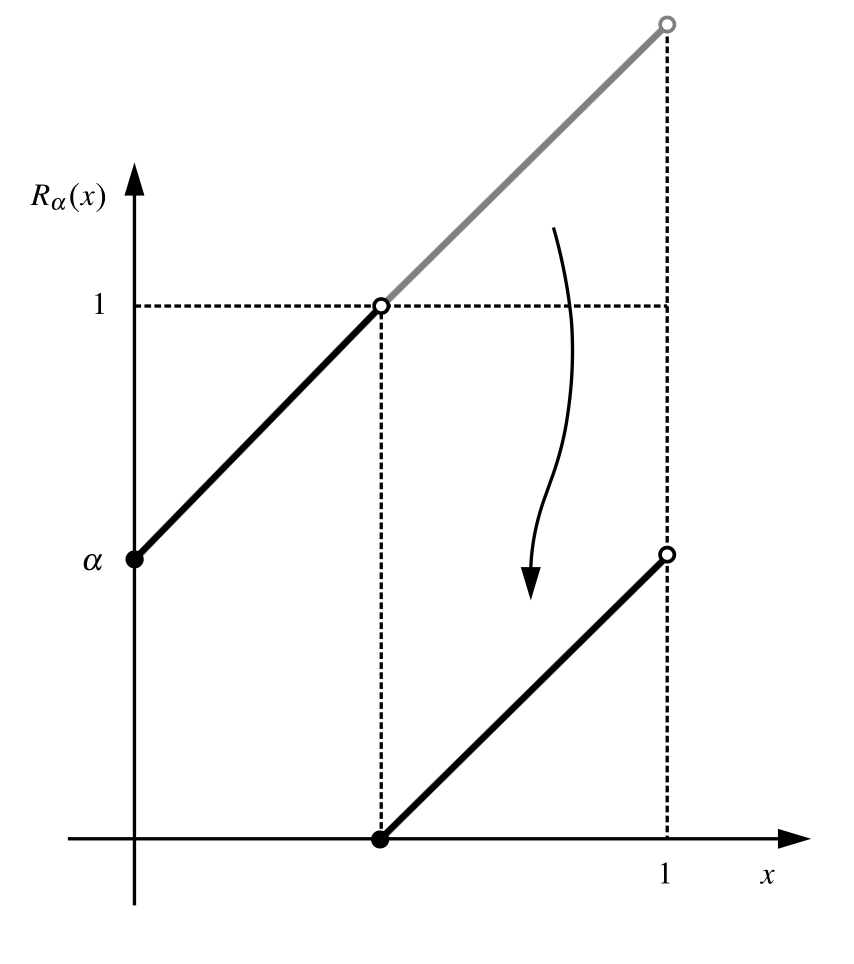
\includegraphics[scale=0.5]{rotacionalpha}
	\end{center}
\end{obsd}

\begin{lem} Sea $\alpha \in \R$.
	\begin{enumerate}[\indent 1)]
		\item Si $\alpha \in \R \setminus \Q$, entonces $R_{\alpha}$ no posee puntos periódicos.
		\item Si $\alpha = \frac{p}{q} \in \Q$ (con $p$ y $q$ coprimos), entonces todos los puntos de $S^{1}$ son periódicos con periodo minimal igual a $q$.
	\end{enumerate}
\end{lem}

\begin{proof}[Idea de la demostración] Observemos que el punto $[x] \in S^{1}$ es periódico de periodo (minimal) $q$ si y solo si
	$$[x + q\alpha] = [x] $$

lo que, por la relación de equivalencia, es equivalente a que 
	$$x + q\alpha - x = q\alpha \in \Z$$

De esta forma, si $\alpha$ es irracional no existen puntos periódicos de ningún periodo. Por otra parte, si $\alpha = \frac{p}{q}$, entonces $q\alpha = p \in \Z$ y todos los puntos son periódicos.
\end{proof}

	%%	Ejemplo con derivada mayor a 1	%%
\subsection{Ejemplo con derivada mayor a 1}
Consideremos ahora una función cuya derivada sea mayor a 1. Sea 
	$$\func{f}{[0,1]}{[0,1]}
		{x}{2x \mod 1}$$
	
Que en un gráfico se ve así
	\begin{center}
		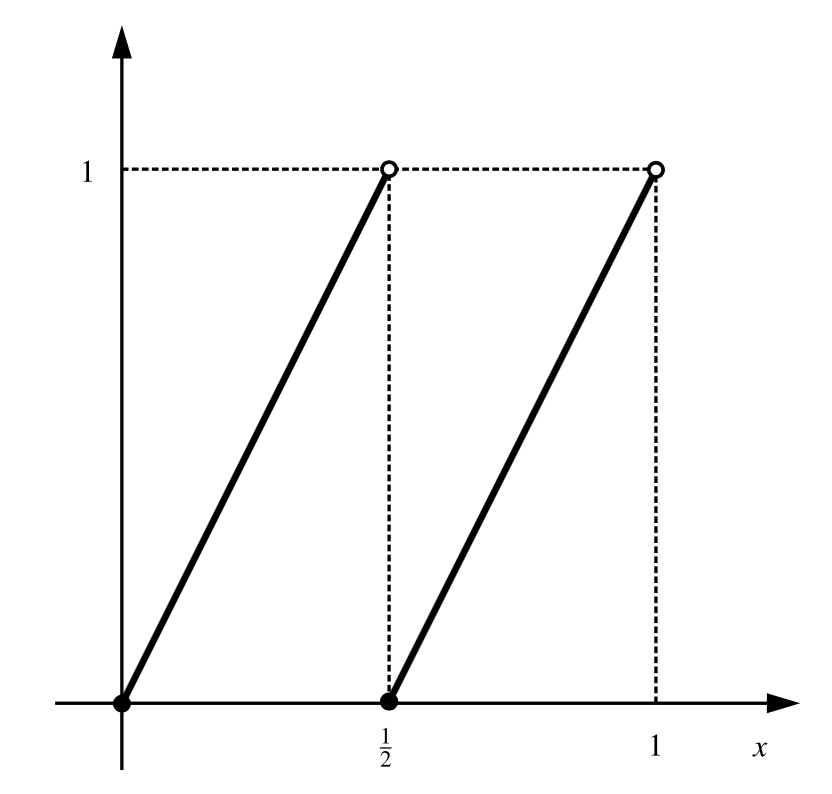
\includegraphics[scale=0.5]{por2mod1}
	\end{center}

En este caso, $x \in [0,1]$ es un punto periódico de periodo $q$ para $f$ si
	$$x = f^{q}(x) = 2^{q}x \mod 1$$

Lo que ocurre si y solo si
	$$2^{q}x - x = (2^{q} - 1)x \in \Z$$

es decir, si existe $p \in \Z$ tal que
	$$x = \frac{p}{2^{q}-1}$$

donde, para que $x \in [0,1]$, $p \leq 2^{q}-1$.

\begin{obs*} Lo que sucedió aquí, de encontrar una ecuación para los puntos periódicos es una rareza y no debe considerarse como la norma.
\end{obs*}

	%%	Full shift en 2 símbolos	%%
\subsection{Full shift en 2 símbolos}
Sea
	$$\Sigma = \{0,1\}^{\N} = \{(x_{i})_{i=1}^{\infty} : x_{i} \in \{0,1\} \} $$

Definimos la función \underline{shift} $\sigma: \Sigma \to \Sigma$ por
	$$\sigma((x_{i})_{i=1}^{\infty}) = (x_{i})_{i=2}^{\infty}$$

\begin{ex} Según lo anterior
	$$\sigma(0011100\ldots) = (011100\ldots)$$
\end{ex}

\begin{ex} Las sucesiones
	\begin{align*}
		\overline{0} = (000\ldots)	\\
		\overline{1} = (111\ldots)
	\end{align*}

son puntos fijos.
\end{ex}

\begin{ex} Las sucesiones $\overline{10}$, $\overline{01}$, $\overline{0}$, $\overline{1}$ son periódicas de periodo 2.
\end{ex}

\begin{ex} Las sucesiones $\overline{000}$, $\overline{001}$, $\overline{010}$, $\overline{011}$, $\overline{100}$, $\overline{101}$, $\overline{111}$ son periódicas de periodo 3.
\end{ex}

En los tres ejemplos anteriores vemos que la cantidad de órbitas periódicas de periodo $n$ eran $2^{n}$. Este hecho se da para los valores de $n$ superiores (Ejercicio).

	%%	Endomorfismos del toro	%%
\subsection{Endomorfismos del toro}
Dado $n \in \N$ definimos el $n$-toro por
	$$\Pi^{n} = \faktor{\R^{n}}{\Z^{n}} = \faktor{\R^{n}}{\sim}$$ 

donde
	$$x \sim y \text{ si y solo si } x-y \in \Z^{n}$$

Los elementos del toro son clases de equivalencia de la forma
	$$[x] = \{x+y : y \in \Z^{n}\}$$

\begin{defn} Sea $A$ una matriz de $n \times n$ con coeficientes en $\Z$. El \rojo{endomorfismo del toro inducido por $A$} corresponde a
	 $$\func{T_{A}}{\Pi^{n}}{\Pi^{n}}
	 			{[x]}{T_{A}([x]) = [Ax]}$$
\end{defn}

\begin{obsd} Como $A$ tiene entradas enteras, entonces $Ax - Ay \in \Z^{n}$ si y solo si $x-y \in \Z^{n}$.
\end{obsd}

\begin{ej}[\href{https://en.wikipedia.org/wiki/Arnold\%27s_cat_map}{Transformación de Arnold (Gato de Arnold)}] Esta transformación se da en $n = 2$ y utiliza
	$$A = \begin{pmatrix}
			2	&	1	\\
			1	&	1
	\end{pmatrix}$$
\end{ej}

\begin{prop} Los puntos periódicos de $T_{A}$ son aquellos con coordenadas racionales (suponga que $A$ es invertible).
\end{prop}

\begin{proof} Tarea
\end{proof}

	%%	Transformación de Gauss	%%
\subsection{Transformación de Gauss}
Definimos la transformación de Gauss por
	$$\func{G}{(0,1]}{(0,1]}
			{x}{\frac{1}{x} - \left[\frac{1}{x}\right]}$$

Que en un gráfico se ve así
	\begin{center}
		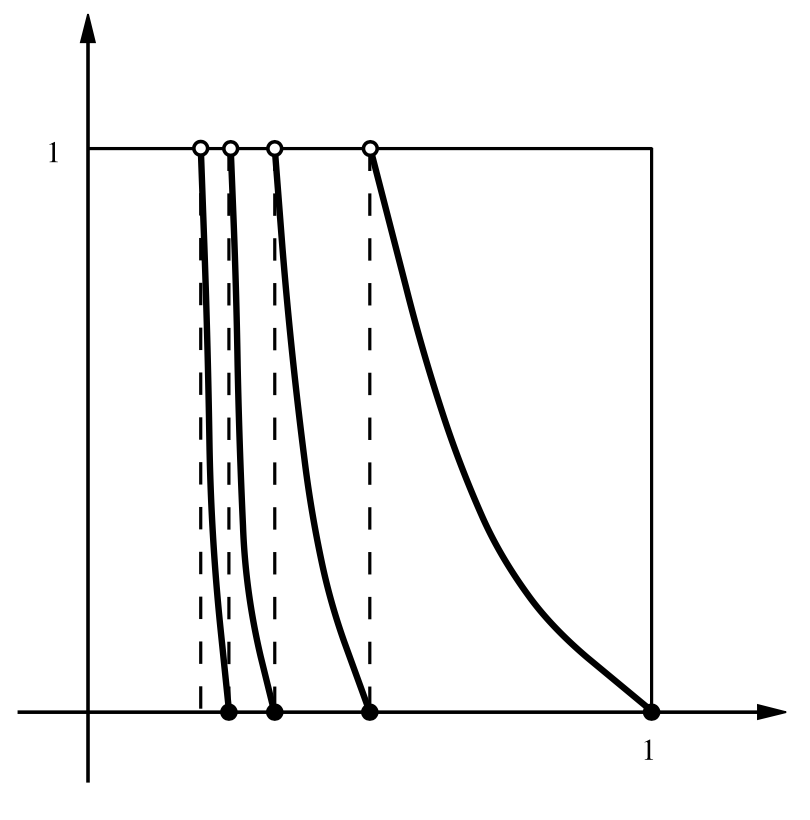
\includegraphics[scale=0.5]{transformaciongauss}
	\end{center}

Esta transformación tiene infinitos puntos fijos. De hecho, $x \in (0,1]$ es punto fijo de $G$ si y solo si
	$$x = [aa \ldots] = \frac{1}{a + \frac{1}{a + \frac{1}{a + \frac{1}{\ddots}}}}$$ 

Observar que como naturalmente tenemos una partición infinita del intervalo (por los números $\frac{1}{n}$), entonces tiene sentido pensar en un alfabeto infinito de símbolos.

\newpage
%%%	Dinámica topológica	%%%
\section{Dinámica topológica}

\begin{defn} Sea $f: X \to X$, con $X$ espacio topológico. El \rojo{$\omega$-límite} de un punto $x \in X$ con respecto a $f$ se define por
	$$\omega(x) = \omega_{f}(x) := \bigcap_{n \in \N} \overline{\{f^{m}(x) : m \geq n\}}$$

Si además $f$ es invertible, el \rojo{$\alpha$-límite} de un punto $x \in X$ con respecto a $f$ se define por
	$$\alpha(x) = \alpha_{f}(x) := \bigcap_{n \in \N} \overline{\{f^{-m}(x) : m \geq n\}}$$
\end{defn}

\begin{prop} Sea $f: X \to X$ y $x \in X$. Entonces $y \in \omega(x)$ si y solo si existe $(n_{k})_{k \in \N}$, subsucesión tal que
	$$\lim_{k \to \infty} f^{n_{k}}(x) = y$$
\end{prop}

\begin{proof} Recordemos que
	$$\omega(x) = \bigcap_{m \geq 1} \overline{A_{m}}$$

donde
	$$A_{m} = \{f^{n}(x) : n \geq m\}$$

Sea $y \in \omega(x)$.
	\begin{casos}
		\item Supongamos que $y \notin \bigcap_{m \geq 1} A_{m}$. Es decir, existe $p \in \N$ tal que $y \notin A_{p}$. Sin embargo, $y \in \overline{A_{p}}$ por definición y por lo tanto $y \in \overline{A_{p}} \setminus A_{p}$ y por lo tanto existe $(n_{k})_{k \in \N}$, con $n_{k} \to \infty$ tal que
				$$\lim_{k \to \infty} f^{n_{k}}(x) = y$$
			
			porque $y$ es punto de acumulación.
			
		\item Supongamos que $y \in \bigcap_{m \geq 1} A_{m}$. Entonces existe $n_{1} \in \N$ tal que
				$$f^{n_{1}}(x) = y$$
			
			Luego, como $y \in A_{m}$ para $m > n_{1}$, entonces existe $n_{2} \in \N$, con $n_{2} > n_{1}$ tal que
				$$f^{n_{2}}(x) = y$$
			
			Continuando de esta manera, obtenemos subsucesión $(n_{k})_{k \in \N}$ y tal que
				$$f^{n_{k}}(x) = y \qquad \paratodo k \in \N$$
			
			lo que implica en particular que
				$$\lim_{k \to \infty} f^{n_{k}}(x) = y$$
	\end{casos}
\end{proof}

\begin{obsp} La idea de esta proposición es que cada punto del $\omega$-límite es un punto al cual la dinámica tiende. 
\end{obsp}

	%%	Rotaciones	%%
\subsection{Rotaciones}

Sea $\alpha \in \Q$. Hemos visto que todo punto $x \in S^{1}$ es periódico bajo esta dinámica. Por lo tanto para todo $x \in S^{1}$ se tiene que $\omega(x)$ es igual a la órbita, en particular es un conjunto finito.	\\

Consideremos ahora $\alpha \in \R \setminus \Q$. En este caso no existen órbitas periódicas.

\begin{lem*} Sea $\alpha \in \R \setminus \Q$. Entonces para todo $x \in S^{1}$, $\omega_{R_{\alpha}}(x) = S^{1}$.
\end{lem*}

\begin{proof} Sea $d$ la métrica en $S^{1}$. Notemos que $R_{\alpha}$ es una isometría. Observemos que si $m_{1} \neq m_{2}$, entonces $R_{\alpha}^{m_{1}}(x) \neq R_{\alpha}^{m_{2}}(x)$. En efecto, supongamos sin pérdida de generalidad que $m_{1} > m_{2} \geq n$ y que $R_{\alpha}^{m_{1}}(x) = R_{\alpha}^{m_{2}}(x)$. Por lo tanto,
	$$x + m_{1}\alpha = x + m_{2}\alpha		\mod 1$$

lo que significa que
	$$m_{1}\alpha - m_{2}\alpha = m \in \Z$$

es decir, $\alpha = \frac{m}{m_{1} - m_{2}} \in \Q$, lo que es una contradicción. En particular, todos los puntos $R^{m}_{\alpha}(x)$, para $m \geq n$ son distintos.	\\

Ahora, sea $\epsilon > 0$ y $N \in \N$ tal que $\frac{1}{N} < \epsilon$. Como todos los puntos
	$$R^{n}_{\alpha}(x), R^{n+1}_{\alpha}(x), \ldots, R^{n+N}_{\alpha}(x)$$

son distintos, existen enteros $0 \leq i_{1} < i_{2} \leq N$ tales que
	$$d(R^{n+i_{1}}_{\alpha}(x), R^{n+i_{2}}_{\alpha}(x)) < \frac{1}{N} < \epsilon$$

por lo que
	$$d(R_{\alpha}^{i_{2} - i_{1}}(x), x) < \epsilon$$

Luego, la sucesión $\{R_{\alpha}^{m(i_{2} - i_{1}}(x)\}_{m \in \N}$ es $\epsilon$-densa. Esto implica que cada órbita es densa, probando lo pedido.
\end{proof}

\begin{ej} Sean $\alpha \in \R \setminus \Q$, $1 \geq \delta > 0$. Demuestre que existen $p \in \Z$ y $q \in \left(0,\frac{1}{\delta}\right] \cap \Z$ tales que
	$$\left| \alpha - \frac{p}{q}\right| < \frac{\delta}{q}$$
\end{ej}

\begin{proof}[Solución] Observar que
	$$\left| \alpha - \frac{p}{q}\right| < \frac{\delta}{q}
		\Longleftrightarrow	|q\alpha - p| < \delta$$
	
Por el lema anterior, la órbita
	$$\{R_{\alpha}(0), R^{2}_{\alpha}(0), \ldots\}$$

es densa en $S^{1}$, de manera que existe un $q \in \N$ (mínimo) tal que
	$$d(0, R^{q}_{\alpha}(0)) < \delta
		\Longleftrightarrow | [q\alpha] - 0| = |[q\alpha]| < \delta$$

Pero $t := [q\alpha] \in [0,1]$ es tal que
	$$q\alpha - t = p \in \Z$$

luego
	$$|q\alpha - p| < \delta$$

que es lo que queríamos probar. Falta ver que $q \leq \frac{1}{\delta}$. Para ello dividamos $S^{1}$ en $q$ ``intervalos'' de igual largo. Consideremos los elementos $\{0, R_{\alpha}(0), \ldots, R_{\alpha}^{q-1}(0)\}$. Necesariamente, existen $0 \leq i < j \leq q-1$ tales que
	 $$|[(j-i)\alpha]| \leq \frac{1}{q}$$

Pero por la minimalidad de $q$, se tiene que
	$$[(j-i)\alpha] \geq \delta$$

de donde se deduce lo deseado.
\end{proof}


	%%	Full shift en 2 símbolos	%%
\subsection{Full shift en 2 símbolos} 
Sea $(\Sigma_{2}, \sigma)$ el full shift en 2 símbolos. Una base para la topología de $\Sigma_{2}$ es la dada por los cilindros.

\begin{defn} Sea $(i_{1}, i_{2}, \ldots, i_{n}) \in \{0,1\}^{n}$. El cilindro $C_{i_{1}, \ldots, i_{n}}$ se define por
	$$C_{i_{1}, \ldots, i_{n}} = \left\{ (x_{i})_{i} \in \Sigma_{2} : x_{1} = i_{1}, x_{2} = i_{2}, \ldots, x_{n} = i_{n}\right\}$$

La colección de todos los cilindros forma una base para la topología de $\Sigma_{2}$.
\end{defn}

\begin{ex} $C_{010} = \{(x_{i})_{i \in \N} : (010\ldots) \}$.
\end{ex}

\begin{obs*} $\Sigma$ es un conjunto de Cantor.
\end{obs*}

Sea $x = (x_{i})_{i} = (0,1,0,0,0,1,1,1,1,\ldots)$. Este punto no es fijo, pero
	$$\sigma^{6}(x) = \sigma^{6+k}(x) = (1,1,1,\ldots)$$

para todo $k \in \N$. Por lo tanto
	$$\omega(x) = \{(1,1,1,\ldots) \}$$

\begin{obs} Los puntos periódicos son densos en $\Sigma$. En efecto, para todo cilindro $C_{i_{1}, \ldots, i_{n}}$ existe un punto periódico $x \in C_{i_{1}, \ldots, C_{i_{n}}}$, de hecho basta tomar $x = (i_{1}, \ldots, i_{n}, i_{1}, \ldots, i_{n}, \ldots)$, es decir, $(\overline{i_{1}, \ldots, i_{n}})$.
\end{obs}

\begin{obs} Existe un punto $(x_{i})_{i} \in \Sigma$ tal que $\omega((x_{i})) = \Sigma$, es decir, existe un punto cuya órbita es densa. Para construir el punto, notemos que la órbita es densa si en cada elemento de la base (los cilindros) encontramos un elemento de la órbita, esa órbita es densa. Construimos el elemento entonces de la siguiente manera
	$$(x_{i}) := (\underbrace{0 \ 1}_{\text{largo 1}} \ \underbrace{00 \ 01 \ 10 \ 11}_{\text{largo 2}} \ \underbrace{000 \ 001 \ 010 \ 100 \ 011 \ 101 \ 110 \ 111}_{\text{largo 3}} \ldots)$$

que contiene, en orden, los (inicios) de los cilindros de largo $k$, para $k \in \N$.
\end{obs}

En este caso tenemos infinitos puntos con órbita densa ya que cualquier permutación del órden (en bloque) de los elementos del punto construido anteriormente sigue manteniendo la propiedad de tener órbita densa. Esto no tiene por qué suceder, como en el siguiente ejemplo.

\begin{ex} Consideremos el sistema dinámico en $[0,1]$ definido por la $f$ del dibujo:
	\begin{center}
		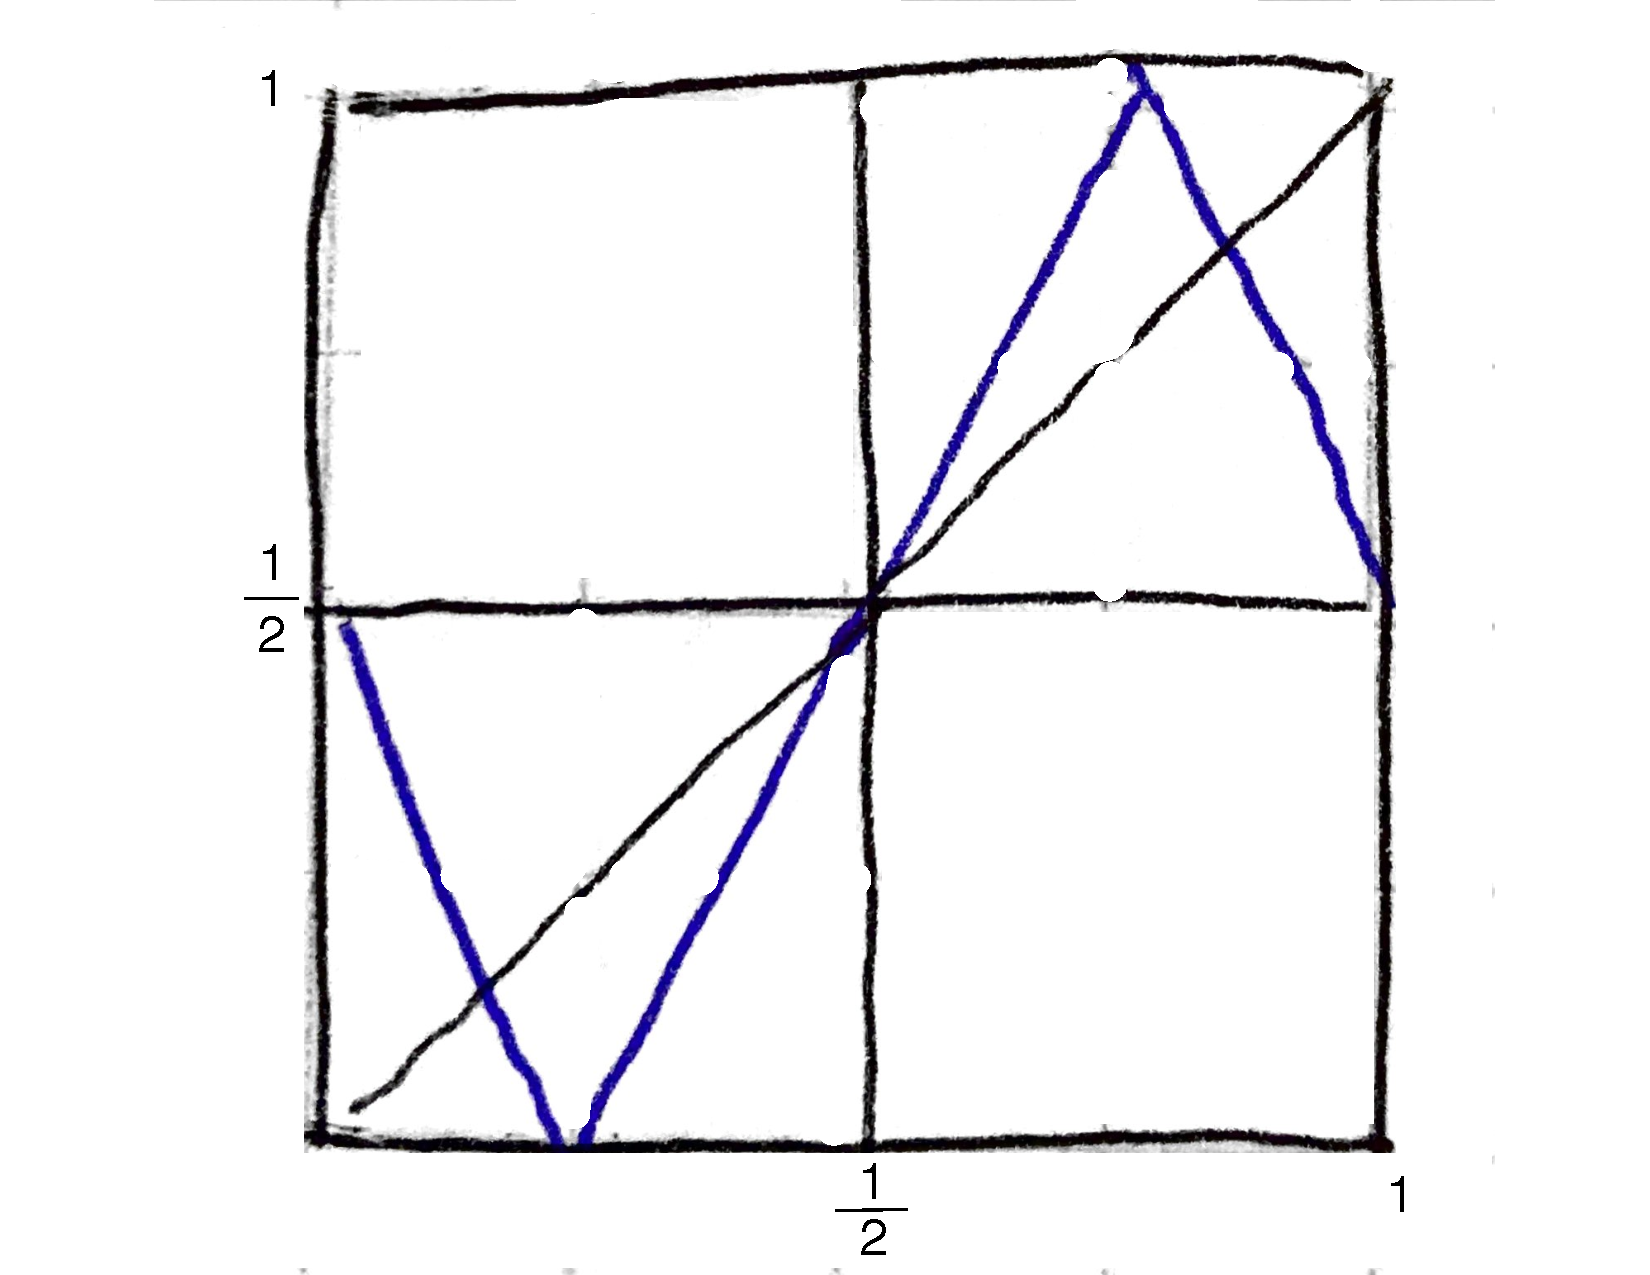
\includegraphics[scale=0.24]{dibujo1}
	\end{center}
	
Como $f([0,1/2]) \subset [0,1/2]$, entonces para todo $x \in [0,1/2]$ la órbita de $x$, que denotaremos por $\gamma(x)$ está contenida en $[0,1/2]$, en particular no es densa.
\end{ex}

	%%	Recurrencia topológica	%%
\subsection{Recurrencia topológica}

\begin{defn} Sea $f: X \to X$ una función continua. Un punto $x \in X$ es \rojo{recurrente} si $x \in \omega(x)$.
\end{defn}

\begin{obsd} Si $x \in X$ es recurrente, entonces existe $(n_{k})_{k \in \N}$ tal que
	$$\lim_{k \to \infty} f^{n_{k}}(x) = x$$
\end{obsd}

\begin{ex} Dado $\alpha \in \R$, todo punto $x \in S^{1}$ es recurrente para $R_{\alpha}$.
\end{ex}

\begin{defn} Un sistema dinámico $f: X \to X$ es \rojo{topológicamente transitivo} si dados $U, V \subset X$ abiertos no vacíos, existe $n \in \N$ tal que $f^{-n}(U) \cap V \neq \emptyset$. 
\end{defn}

\begin{teo} Sea $f: X \to X$ continua y $X$ compacto y separable (con base numerable).
	\begin{enumerate}[\indent 1)]
		\item Si $f$ es topológicamente transitivo, entonces existe $x \in X$ cuya órbita es densa en $X$.
		
		\item Si $X$ no posee puntos aislados y existe $x \in X$ con órbita densa, entonces $f$ es topológicamente transitivo.
	\end{enumerate}
\end{teo}

\begin{proof}[Demostración de 1)] Supongamos que $f$ es topológicamente transitivo. Sea $U \neq \emptyset$ abierto. El conjunto
	$$\bigcup_{n=0}^{\infty} (f^{-n}U)$$

es (abierto y) denso en $X$ por hipótesis. En efecto, dado $V \subset X$ abierto, por hipótesis existe $N \in \N$ tal que $f^{-N}U \cap V \neq \emptyset$. Esto implica que
	$$V \cap \bigcup_{n=0}^{\infty} (f^{-n}U) \neq \emptyset$$

mostrando que el conjunto es denso. Sea $(U_{i})_{i \in \N}$ la base numerable de la topología de $X$. Este es un espacio de Baire, de manera que
	$$Y := \bigcap_{i \in \N} \bigcup_{n \in \N} f^{-n}(U_{i}) \neq \emptyset$$

Sea $x  \in Y$, tenemos que $x \in \bigcup_{n \in \N} f^{-n}U_{i}$ para cada $i \in \N$, por lo tanto
	$$\{x, f(x), f^{2}(x), \ldots, f^{n}(x), \ldots\} \cap U_{i} \neq \emptyset$$

Como esto sucede para todo elemento de la base, entonces la órbita de $x$ es densa en $X$.
\end{proof}

\begin{proof}[Demostración de 2)] Supongamos que $X$ no posee puntos aislados y que existe $x \in X$ con órbita densa. Sean $U, V \subset x$ abiertos no vacíos. La órbita de $x$, por ser densa, intersecta en infinitos puntos tanto a $U$ como a $V$. En particular existen $m > n \in \N$ tales que
	$$f^{m}(x) \in U, \, f^{n}(x)  \in V$$

Luego 
	$$x \in f^{-m}(U) \cap f^{-n}(V) = f^{-n}\left(f^{-(m-n)}(U) \cap V \right)$$. 

De manera que
	$$f^{-(m-n)}(U) \cap V \neq \emptyset$$
	
y por lo tanto $f$ es topológicamente transitivo.
\end{proof}

\begin{obst} Si $f: X \to X$ es topológicamente transitivo, entonces existe un punto con órbita densa. Esto implica que no se puede separar el sistema dinámico en piezas para estudiarlas independientemente. En ese sentido, ser topológicamente transitivo es una condición de irreducibilidad.
\end{obst}

\begin{defn} Un sistema $f: X \to X$ es \rojo{topológicamente mezclante (mixing)} si dados abiertos no vacíos $U,V \subset X$ existe $n \in \N$ tal que para todo $m \geq n$ se tiene
	$$f^{-m}(U) \cap V \neq \emptyset$$
\end{defn}

\begin{obsd} Toda transformación topológicamente mixing es topológicamente transitiva. Sin embargo el recíproco no es cierto.
\end{obsd}

\begin{ex} Sea $\alpha \in \R \setminus \Q$ y $\R_{\alpha}$ la rotación en ángulo $\alpha$. Como toda órbita es densa, $R_{\alpha}$ es topológicamente transitiva. Sin embargo, sea $\epsilon < \frac{1}{4}$ y consideremos el abierto
	$$U := (x-\epsilon, x+\epsilon) \subset S^{1}$$

como $\epsilon < \frac{1}{4}$, entonces este abierto queda contenido en una mitad de $S^{1}$. Además, cada preimagen $U$ es un intervalo abierto de largo $2\epsilon < \frac{1}{2}$. Como la órbita de $x$ es densa, existe subsucesión $(n_{k})_{k}$ tal que
	$$R_{\alpha}^{n_{k}}(x) \tiende{n} x + \frac{1}{2}$$

Luego
	$$R_{\alpha}^{n_{k}}(U) \cap U = \emptyset$$
	
para infinitos valores de $k$ y por lo tanto no es topológicamente mixing.
\end{ex}

\begin{ej} Sea $(\Sigma_{2}, \sigma)$ el full shift en 2 símbolos. Demostrar que es topológicamente mixing.
\end{ej}

\begin{proof}[Solución] Basta probar la propiedad de topológicamente mixing para los elementos de la base de la topología de $\Sigma_{2}$. Sean $U = C_{i}, V= C_{j}$ dos cilindros, con $i = (i_{1} \cdots i_{N_{1}})$, $j = (j_{1}, \ldots, j_{N_{2}})$. Sea $n := N_{2}$ en la definición, para $m \geq n = N_{2}$ tenemos que el elemento 
	$$x_{m} = (j_{1}, \ldots, j_{N_{2}}, \ldots, j_{m}, i_{1}, \ldots, i_{N_{1}}, 0, 0, \ldots) $$

pertenece a $V$ y además $\sigma^{m}(x_{m}) = (i_{1}, \ldots, i_{N_{1}}, 0 , 0, \ldots) \in U$, por lo que $x_{m} \in f^{-m}(U) \cap V$.
\end{proof}


	%%	Entropía topológica %%
\subsection{Entropía topológica}

Sea $(X,d)$ un espacio métrico compacto. Sea $T: X \to X$ una transformación continua. Para $n \in \N$ definimos la siguiente métrica (ejercicio) en $X$:
	$$d_{n}(x,y) := \max_{i \in \{0,\ldots,n-1\}} d(T^{i}x, T^{i}y) $$

\begin{obs} Esta métrica en cierto sentido está midiendo la distancia entre órbitas, hasta tiempo $n$ y preservando este tiempo, es decir, podría ser que $T^{j}y$ esté muy cerca de $x$ para cierto $j$, pero no nos interesa esa distancia en particular.
\end{obs}

\begin{obs} La bola de centro $x \in X$ con la métrica $d_{n}$ viene dada por:
	$$B_{d_{n}}(x,r) = \bigcap_{i=1}^{n} T^{-i}(B(T^{i}x,r))$$

Los puntos de esta bola son aquellos que se mantienen dentro de las bolas de radio $r$ alrededor de cada $T^{i}x$, con $i = 0, \ldots, n-1$. 
\end{obs}

\begin{defn} Sea $n \in \N$, $\epsilon > 0$. Un subconjunto $F$ de $X$ es \rojo{$(n,\epsilon)$-generador con respecto a $T$} si y solo si para todo $x \in X$ existe $y \in F$ tal que $d_{n}(x,y) < \epsilon$.
\end{defn}

\begin{obsd} Básicamente, un $F$ es $(n,\epsilon)$-generador si para cada punto de $X$, la órbita de ese punto está arbitrariamente cerca (distancia $\epsilon$) de la órbita de algún $y \in F$, hasta tiempo $n$.	\\

Analogamente, un $F$ es $(n,\epsilon)$-generador si las bolas (en la métrica $d_{n}$) de radio $\epsilon$ alrededor de cada $y \in F$ cubren a $X$. Esta interpretación es importante porque el espacio es compacto y las bolas son abiertas.
\end{obsd}

\begin{defn} Sea $n \in \N$ y $\epsilon > 0$. Denotaremos por $r_{n}(\epsilon)$ a la menor cardinalidad de cualquier conjunto $(n,\epsilon)$-generador.
\end{defn}

\begin{obsd} Como el espacio es compacto $r_{n}(\epsilon) < \infty$ para cada $n \in \N, \epsilon > 0$. En efecto, como dijimos antes, si $F \subset X$ es $(n,\epsilon)$-generador, entonces el cubrimiento dado por bolas $B_{d_{n}}(x,\epsilon)$, con $x \in F$ posee un sub-cubrimiento finito. En particular existe $F' \subset F$ finito y $(n,\epsilon)$-generador.
\end{obsd}

\begin{obsd} Si $\epsilon_{1} < \epsilon_{2}$, entonces $r_{n}(\epsilon_{1}) \geq r_{n}(\epsilon_{2})$. Es decir, entre más fina es mi separación ``más órbitas distintas'' se ven.
\end{obsd}

\begin{defn} Sea $\epsilon > 0$, definimos
	$$r(\epsilon) := \limsup_{n \to \infty} \frac{1}{n} \log r_{n}(\epsilon)$$
\end{defn}

\begin{obsd} Al definir esto, entonces estamos diciendo que
	$$r_{n}(\epsilon) \sim e^{n r(\epsilon)}$$

\end{obsd}

\begin{obsd} Si $\epsilon_{1} < \epsilon_{2}$, entonces $r(\epsilon_{1}) \geq r(\epsilon_{2})$, lo que es esperable de la observación anterior.
\end{obsd}

\begin{obsd} Es posible que $r(\epsilon) = +\infty$.
\end{obsd}

\begin{defn} La \rojo{entropía topológica} de una transformación continua $T: X \to X$, donde $X$ es compacto, viene dada por
	$$h(T) := \lim_{\epsilon \to 0} r(\epsilon)$$
\end{defn}

\begin{ex}[Rotaciones] Sea $\alpha \in \R$ y $R_{\alpha}: S^{1} \to S^{1}$ la rotación asociada. Observar que como la rotación es una isometría,
	$$d(R^{n}_{\alpha}(x), R^{n}_{\alpha}(y)) = d(R_{\alpha}(x), R_{\alpha}(y)) = d(x,y) \qquad \paratodo n \in \N$$

de manera que $d_{n} = d$ para todo $n \in \N$. Luego
	$$h(R_{\alpha}) = \lim_{\epsilon \to 0} \limsup_{n \to \infty} \frac{1}{n} \log r_{n}(\epsilon)$$

pero $r_{n}(\epsilon) = r_{1}(\epsilon)$ y por lo tanto
	$$h(R_{\alpha}) = \lim_{\epsilon \to 0} \limsup_{n \to \infty} \frac{1}{n} \log r_{1}(\epsilon) = 0$$
\end{ex}

\begin{obsex} En general, si $T$ es una isometría, entonces $h(T) = 0$.
\end{obsex}

A continuación daremos una definición dual de la entropía, en el sentido siguiente. La definición anterior intentaba ``juntar'' o ``cubrir'' todo $X$. Ahora buscaremos ``separar'' $X$.

\begin{defn} Sea $n \in \N$ y $\epsilon > 0$. Un subconjunto $E \subset X$ es \rojo{$(n,\epsilon)$-separado con respecto a $T$} si para cada $x,y \in E$, $x \neq y$, $d_{n}(x,y) > \epsilon$.  
\end{defn}

\begin{defn} Sean $n \in \N$, $\epsilon > 0$. Denotamos por $s_{n}(\epsilon)$ a la mayor cardinalidad de cualquier conjunto $(n,\epsilon)$-separado con respecto a $T$
\end{defn}

\begin{obsd} Si $\epsilon_{1} < \epsilon_{2}$, entonces $s_{n}(\epsilon_{1}) \geq s_{n}(\epsilon_{2})$.
\end{obsd}

\begin{ej} $r_{n}(\epsilon) \leq s_{n}(\epsilon) \leq r_{n}\left(\frac{\epsilon}{2}\right)$.
\end{ej}

\begin{proof}[Solución] Sea $E \subset X$ $(n,\epsilon)$-separado con respecto a $T$ y $|E| = s_{n}(\epsilon)$. Sea $F \subset X$ $\left(n,\frac{\epsilon}{2}\right)$-generador con respecto a $T$ y de cardinalidad $|F| = r_{n}\left(\frac{\epsilon}{2}\right)$. Para cada $y \in E$ existe $x_{y} \in F$ con $d(x_{y}, y) < \frac{\epsilon}{2}$. Además, si $y_{1}, y_{2} \in E$, con $y_{1} \neq y_{2}$, entonces $x_{y_{1}} \neq x_{y_{2}}$ pues
	$$\epsilon < d(y_{1}, y_{2}) \leq d(y_{1}, x_{y_{1}}) + d(x_{y_{1}}, x_{y_{2}}) + d(x_{y_{2}}, y_{2}) < \epsilon + d(x_{y_{1}}, x_{y_{2}})$$

de donde $d(x_{y_{1}},x_{y_{2}}) > 0$, mostrando que $x_{y_{1}} \neq x_{y_{2}}$. Esto implica que la asignación $y \mapsto x_{y}$ es inyectiva y por lo tanto 
	$$s_{n}(\epsilon) = |E| \leq |F| = r _{n}\left(\frac{\epsilon}{2}\right)$$

Para la otra desigualdad, sea $F \subset X$ ahora $(n,\epsilon)$-generador con respecto a $T$, con cardinalidad $|F| = r_{n}(\epsilon)$. Observar que como $|F|$ tiene la menor cardinalidad posible, entonces no ocurre que una cierta bola $B_{d_{n}}(x,\epsilon)$ no puede estar cubierta por otra bola ni por uniones de otras bolas (porque si así fuera podríamos quitar a $x$ de $F$ y $F\setminus\{x\}$ sería $(n,\epsilon)$-generador). 
\end{proof}


\begin{obsej} Esto dice en particular que $s_{n}(\epsilon) < \infty$ para cada $n \in \N$, $\epsilon > 0$.
\end{obsej}

\begin{defn} Sea $\epsilon > 0$, definimos
	$$s(\epsilon) = \limsup_{n \to \infty} \frac{1}{n} \log s_{n}(\epsilon)$$
\end{defn}

\begin{defn} La entropía topológica de $T$ se puede definir por
	$$h(T) = \lim_{\epsilon \to 0} s(\epsilon)$$

y coincide con la definición anterior.
\end{defn}

\begin{ex} Calcularemos la entropía topológica del full shift en dos símbolos, es decir $(\Sigma, \sigma)$ con $\Sigma = \{(x_{i})_{i=1}^{\infty} : x_{i} \in \{1,2\}\}$ y
	$$\func{\sigma}{\Sigma}{\Sigma}
				{(x_{1}, x_{2}, \ldots)}{x_{2}, x_{3}, \ldots,}$$

Consideremos la siguiente métrica en $\Sigma$:
	$$d((x_{i})_{i}, (y_{i})_{i}) = \frac{1}{2^{\min\{i : x_{i} \neq y_{i}\}}}$$

por ejemplo,
	$$d((000110\ldots), (00010\ldots)) = \frac{1}{2^{3}}$$

porque el tercer símbolo es el primero en el que difieren. Observemos que el espacio $(\Sigma, d)$ es compacto (es un conjunto de Cantor). La entropía se calcula
	$$h(\sigma) = \lim_{\epsilon \to 0} \limsup_{n \to \infty} \frac{1}{n} \log s_{n}(\epsilon)$$
	
Comencemos con $\epsilon = \frac{1}{2}$ y calculemos $s_{n}(\epsilon)$. La métrica a considerar es
	$$d_{n}(x,y) = \max \{d(\sigma^{i}x, \sigma^{i}y) : i \in \{0, \ldots, n-1\}\}$$

Observar que $d(x,y) \leq \frac{1}{2}$ si y solo si $x_{1} = y_{1}$. De esta manera, si queremos $d_{2}(x,y) \leq \frac{1}{2}$, entonces $d(x,y) \leq \frac{1}{2}$ y $d(\sigma x, \sigma y) \leq \frac{1}{2}$, es decir, debe ocurrir que $x_{1} = y_{1}$ y $x_{2} = y_{2}$. De la misma forma, $d_{2}(x,y) \leq \frac{1}{2}$ si y solo si
	\begin{itemize}
		\item $d(x,y) \leq \frac{1}{2}$, si y solo si $x_{1} = y_{1}$.
		\item $d(\sigma x,\sigma y) \leq \frac{1}{2}$ si y solo si $x_{2} = y_{2}$.
		\item $d(\sigma^{2} x, \sigma^{2}y) \leq \frac{1}{2}$ si y solo si $x_{3} = y_{3}$.
	\end{itemize}

Vemos que lo que ocurre es que la métrica $d_{n}$ genera cilindros de ``tamaño'' $n$. Como a cada paso $n$, tenemos $2^{n}$ cilindros, entonces a lo más hay $2^{n}$ puntos $(n,\epsilon)$ separados (cualquier otro está en algun cilindro que ya contiene a alguno de esos $2^{n}$ puntos), es decir,
	$$s_{n}(\epsilon) = 2^{n}$$

En efecto, consideremos el conjunto
	$$I_{2} = \{(0000\ldots), (010101\ldots), (101010\ldots), (111111\ldots) \}$$

este conjunto es $(2,\epsilon)$-separado y tiene la cardinalidad máxima pues cualquier otro punto $x \in \Sigma$ debe pertenecer a alguno de los cuatro cilindros y cada uno de los puntos de $I_{2}$ pertenece a un cilindro distinto. Esto nos indica que $\epsilon$ no juega un rol tan importante en esto. En general, si $\epsilon < \frac{1}{2}$, entonces tendremos que $s_{n}(\epsilon) = 2^{n+k}$ donde $k$ depende de $\epsilon$ (si $\epsilon$ es muy pequeño tenemos que pedir más cilindros para encontrar los puntos anteriores) pero no depende de $n$. Luego
	$$h(\sigma) = \lim_{\epsilon \to 0} \lim_{n \to \infty} \frac{1}{n} \log 2^{n+k} = \log 2$$
\end{ex} 

	%% Conjugación topológica %%
\subsection{Conjugación topológica}
\begin{defn} Sean $f: X \to X$, $g: Y \to Y$ dos funciones continuas definidas en compactos $X,Y$. Diremos que un homeomorfismo $H: X \to Y$ es una \rojo{conjugación topológica} entre $f$ y $g$ si (y solo si) el diagrama
	$$\begin{array}{ccc}
		X			&	\xrightarrow{\quad f \quad}	&	X	\\
		\downarrow H	&							&	\downarrow H	\\
		Y			&	\xrightarrow{\quad g \quad}	&	Y
	\end{array}$$

es conmutativo, es decir $H \circ f = g \circ H$.
\end{defn}

\begin{obsd} Si $f(p) = p$, entonces $H(p)$ es un punto fijo de $g$. En efecto
	$$g(H(p)) = H(f(p)) = H(p)$$

Lo mismo ocurre con puntos periódicos. En efecto, como $H$ es invertible
	$$g = H^{-1} \circ f \circ H$$

luego
	$$g^{n} = H^{-1} \circ f^{n} \circ H$$

y como los puntos periódicos de largo $n$ para $f$ son fijos para $f^{n}$, entonces obtenemos el resultado. Más aún el resultado dice que los periodos son iguales.
\end{obsd}

\begin{ex} Los sistemas $(\Sigma_{2}, \sigma)$ y $(\Sigma_{3}, \sigma)$ no son topológicamente conjugados. Si existiera tal conjugación, entonces tendríamos una biyección entre los puntos fijos de cada uno. Sin embargo, $(\Sigma_{2}, \sigma)$ tiene 2 puntos fijos (a saber, $\overline{0}$ y $\overline{1}$), mientras que $(\Sigma_{3}, \sigma)$ posee 3 puntos fijos (a saber, $\overline{0}$, $\overline{1}$, $\overline{2}$).
\end{ex}

\begin{ex} Los sistemas $(S^{1}, R_{1/3})$ y $(S^{1}, R_{1/4})$ no son topológicamente conjugados, pues en el primero los periodos son de largo 3 y en los segundos son de largo 4. Como los periodos deben tener el mismo largo, no son existe conjugación topológica.
\end{ex}

\begin{teo} La entropía topológica es un invariante bajo conjugación topológica.
\end{teo}

\begin{proof}[Demostración 1] Sean $f: X \to X$, $g: Y \to Y$ funciones continuas definidas en compactos y $H:X \to Y$ conjugación topológica. Sea $d$ una métrica que genera la topología en $X$. Definimos en $Y$ la siguiente métrica
	$$d'(y_{1}, y_{2}) := d(H^{-1}(y_{1}), H^{-1}(y_{2}))$$

Luego $H: (X,d) \to (Y, d')$ es una isometría y por lo tanto conjuntos $(n,\epsilon)$-separados en $X$ para $f$ se mapean en conjuntos $(n,\epsilon)$-separados en $Y$ para $g$.
\end{proof}

	%%	Ejemplo: Flujos de suspensión %%
\subsection{Ejemplo: Flujos de suspensión}
Sea $(X,T)$ un sistema dinámico a tiempo discreto (acción viene dada por $\N$ o $\Z$). Sea $\clx{T}: X \to \R^{+}$ una función continua y positiva tal que existe $\alpha > 0$, de modo que para todo $x \in X$, se tiene $\clx{T}(x) \geq \alpha > 0$. Definimos el espacio
	$$\tilde{Y} := \{(x,t) : x \in X, \, t \in [0,\clx{T}(x)] \}$$

e identificamos (pegamos) los puntos $(x, \clx{T}(x))$ con $(T(x), 0)$, es decir $(x, \clx{T}(x)) \sim (Tx, 0)$ e
	$$Y = \faktor{\tilde{Y}}{\sim}$$

El flujo de suspensión $\Phi = (\varphi_{t})_{t \in \R}$ sobre $(X,T)$ con techo $\clx{T}$ se define por
	$$\varphi_{r}(x, t) = (x, t+r)$$

si $0 < t+r < \clx{T}(x)$.	\\

Observemos que si $\{x, Tx, \ldots, T^{n-1}x\}$ es una órbita periódica de $T$ de periodo $n$, entonces la órbita del flujo es periódica y el periodo de esa órbita es $\clx{T}(x) + \clx{T}(Tx) + \cdots + \clx{T}(T^{n-1}x)$. Podemos pensar que este modelo trata de simplificar lo siguiente.	\\

Supongamos un flujo de vector en un espacio (si queremos, $\R^{3}$). Supongamos que tenemos un cierto corte transversal (no necesariamente infinito) de ese espacio. El vector, si el corte transversal es suficientemente bueno, pasa por el corte transversal una cantidad infinita de veces y cada vez que lo corta podemos pensar que estamos en un sistema dinámico discreto y los cortes son la órbita del vector $x$. En ese sentido, el tiempo que se demora el vector al pasar desde $x$ a $Tx$ corresponde a $\clx{T}(x)$.

	%% Ejemplo: Smeale's Horseshoe (Herradura de Smeale) %%
\subsection{Ejemplo: Smale's Horseshoe (Herradura de Smale)}
Consideremos el cuadrado $[0,1] \times [0,1]$. Vamos a aplastarlo, estirarlo y doblarlo para luego incrustarlo en el cuadrado original:
	\begin{center}
		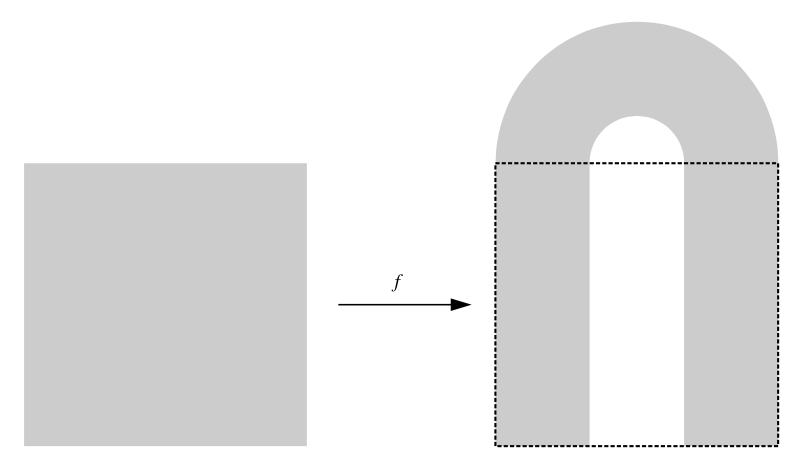
\includegraphics[scale=0.5]{horseshoe1}
	\end{center}

Evidentemente no puedo componer el cuadrado consigo mismo, porque la imagen no está completamente metida en el cuadrado original. Pero podemos quedarnos solamente con la parte que sí está. Lo que resulta termina siendo $\rmx{Cantor}_{1/3} \times [0,1]$, es decir, una peineta cuyos dientes son de largo 1 ubicados en los puntos del conjunto de Cantor. Si hacemos lo mismo con $f^{-1}$ (preimágenes), entonces obtenemos $[0,1] \times \rmx{Cantor}_{1/3}$.	\\

Observemos que el conjunto $\Lambda = \{x \in [0,1]^{2} : f^{n}(x) \text{ está bien definido para todo } n \in \Z\}$ es $C_{1/3} \times C_{1/3}$. Luego, $(f, \Lambda)$ es topológicamente conjugado a $(\Sigma_{2}, \sigma)$, el full shift en 2 símbolos.	\\

Este sistema tiene dos puntos fijos (Ejercicio).

\newpage
%%%	Dinámica uno dimensional	%%%
\section{Dinámica uno dimensional}

Sea $f: \R \to \R$ definida por $f(x) = x^{2}$. Observemos que del gráfico
	% escribir parábola en TikZ con la recta y = x
	\begin{center}
	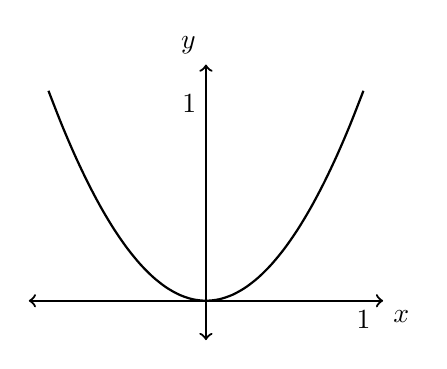
\begin{tikzpicture}[scale =0.5]
		\draw[thick, <->] (0,-1) -- (0,6) node[anchor=south east] {$y$};
		\draw[thick, <->] (-4.5,0) -- (4.5,0) node[anchor=north west] {$x$}; 
		\node[below] at (4 ,0) {1};
		\node[left] at (0,5) {1};
		\draw[thick, domain=-4:4,smooth,variable=\x] plot ({\x},{\x*\x/3});
	\end{tikzpicture}
	\end{center}
	
los únicos puntos fijos son $x = 0$ y $x = 1$. Además $x = -1$ es eventualmente fijo, ya que $f(-1) = 1$, que es fijo. Evidentemente, si $|x| > 1$, entonces $f^{n}(x) \tiende{n} \infty$. Como además, $f(x) \geq 0$ para cada $x$, entonces la parte interesante de la dinámica (o solamente la dinámica) está en $[0,1]$.
	% dibujar cuadrado [0,1] x [0,1] con la recta y= x y el pedazo de parabola

Observar que para todo $x \in [0,1)$ se tiene que $\lim_{n \to \infty} f^{n}(x) = 0$.

\begin{defn} Sea $f: \R \to \R$ de clase $C^{N}$, para un $N$ conveniente. Un punto de periódico de periodo $n$ se dice \rojo{hiperbólico} si $|(f^{n})'(p)| \neq 1$.
\end{defn}

\begin{lem} Sea $p$ un punto fijo tal que $|f'(p)| < 1$, entonces existe un intervalo $U$ tal que $p \in U$ y si $x \in U$, entonces
	$$\lim_{n \to \infty} f^{n}(x) = p$$
\end{lem}

\begin{proof} Como $f \in C^{1}$, entonces existe $\epsilon > 0$ tal que $|f'(x)| < A < 1$. Para $x \in [p-\epsilon, p+\epsilon]$. Por TVM
	$$|f(x) - p| = |f(x) - f(p)| \leq A (x - p) < (x-p) < \epsilon$$

Luego, si $x \in [p-\epsilon, p +\epsilon]$, entonces $f(x)  \in [p-\epsilon, p + \epsilon]$. Repitiendo el argumento $n$ veces tenemos que
	$$|f^{n}(x) - p| \leq A^{n}|x-p|$$

como $A < 1$, entonces $\lim_{n \to \infty} f^{n}(x) = p$.
\end{proof}

\begin{defn} Sea $p$ un punto periódico de periodo $n$ tal que $|(f^{n})'(p)| < 1$. Diremos que $p$ es un punto periódico \rojo{atractor}.
\end{defn}

\begin{lem} Sea $p$ un punto fijo tal que $|f`(p)| > 1$. Entonces existe una vecindad $U$ de $p$ tal que si $x \neq p$, entonces existe $k \in \N$ tal que $f^{k}(x) \notin U$.
\end{lem}

\begin{defn} Diremos que un punto fijo $p$ tal que $|f'(p)| > 1$ es un \rojo{repulsor}.
\end{defn}

	%%	Ejemplo: Familia cuadrática	%%
\subsection{Ejemplo: Familia cuadrática}
Sea $\mu > 0$. Sea $F: [0,1] \to [0,1]$ definida por $F(x) = \mu x(1-x)$. Observemos que $F_{\mu}$ posee un máximo en $x= \frac{1}{2}$. Tenemos que $F_{\mu}(0) = 0$ por lo que 0 es punto fijo para todo $\mu$. Pero además
	$$F_{\mu}'(x) = \mu - 2\mu x$$
 
por lo que $F'_{\mu}(0) = \mu$. De esta manera, si $\mu \in (0,1)$, entonces existe un único punto fijo $p = 0$ y es un atractor. Si $\mu > 1$, entonces $p_{1} =0$ es repulsor y más aún hay otro punto fijo que es $p_{2} = \frac{\mu - 1}{\mu}$ con
	$$F'_{\mu}\left(\frac{\mu-1}{\mu}\right) = 2- \mu $$

Luego, si $\mu \in (1,3)$, entonces $|F'_{\mu}(p_{2})| < 1$ y por lo tanto $p_{2}$ es atractor, si $\mu > 3$, entonces $p_{2}$ es repulsor.	\\

Si $\mu = 4$, entonces $F_{4}$ se suele llamar aplicación de Ulam-Von Neumann y es topológicamente conjugado con $2x \mod 1$ o bien a $(\Sigma_{2}, \sigma)$ (Ejercicio de prueba). En particular $h(F_{4}) = \log 2$.	\\

Observar ahora que si $\mu > 4$ entonces hay puntos para los cuales $F_{\mu}(x) > 1$, en particular esos puntos no pueden ser iterados más de una vez. Es decir, el conjunto $\Lambda = \conj{x \in [0,1]}{F_{\mu}^{n}(x) \text{ está definido } \paratodo n \in \N}$ es un conjunto de Cantor. En particular $h(F_{\mu}) = \log 2$ para $\mu > 4$.


	%%	Homeomorfismos del círculo	%%
\subsection{Homeomorfismos del círculo}

\begin{defn} Un levantamiento (lift) de un homeomorfismo del círculo $f: S^{1} \to S^{1}$ es una función continua $F: \R \to \R$ tal que
	$$f \circ \pi = \pi \circ F$$

donde $\pi : \R \to S^{1}$ es la proyección natural, es decir, $\pi(x) = [x]$. 
\end{defn}

\begin{obsd} Basta considerar el representante en $[0,1)$ de la clase de equivalencia $[x]$, es decir, $\{x\} = x - \lfloor x \rfloor$.
\end{obsd}

\begin{obsd} Se tiene el siguiente diagrama conmutativo:
	$$\begin{array}{ccc}
		\R			&	\xrightarrow{\quad F \quad}	&	\R	\\
		\downarrow \pi	&							&	\downarrow \pi	\\
		S^{1}		&	\xrightarrow{\quad f \quad}	&	S^{1}
	\end{array}$$
\end{obsd}

En un gráfico, un lift se ve así:
	\begin{center}
		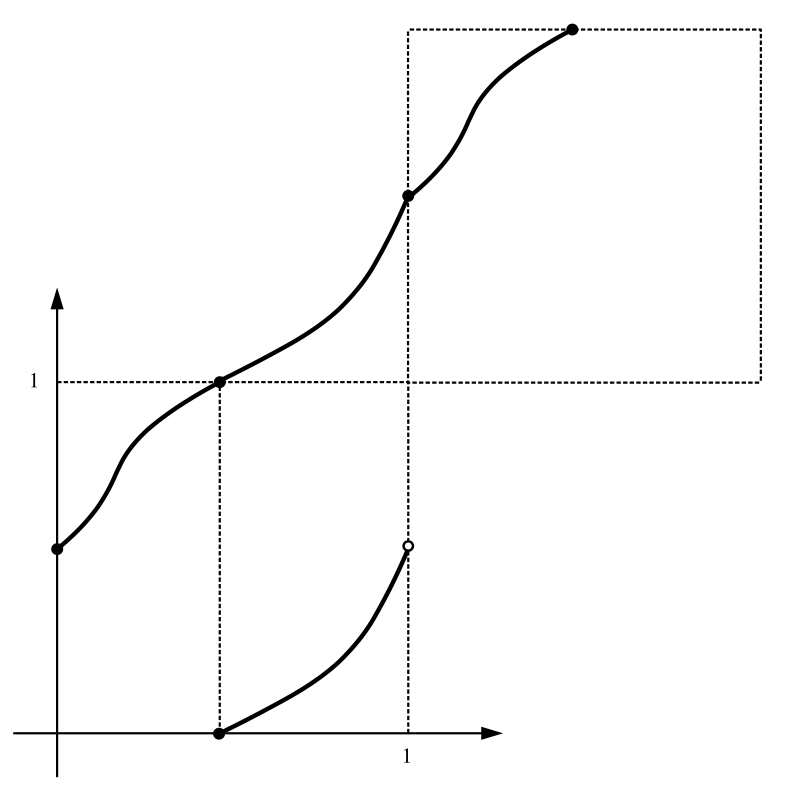
\includegraphics[scale=0.5]{lift}
	\end{center}

\begin{ex} Sea $\alpha \in \R$, $R_{\alpha}: S^{1} \to S^{1}$ la rotación en ángulo $\alpha$,
	$$R_{\alpha}(x) = x+\alpha \mod 1$$

Dado $k \in \Z$, considere la función
	$$\func{F}{\R}{\R}
			{x}{x + \alpha + k}$$
		
La función $F$ es un levantamiento de $R_{\alpha}$. En efecto
	\begin{align*}
		\pi(F(x))
			&=	\pi(x + \alpha + k)	\\
			&=	x + \alpha + k \mod 1	\\
			&=	\pi(x) + \alpha \mod 1	\\
			&=	R_{\alpha}(\pi(x))
	\end{align*}

Evidentemente aquí $k$ no jugó ningún rol, salvo ser entero. Luego tenemos infinitos levantamientos (o uno salvo por un entero)
\end{ex}

\begin{ex} Sea $\beta \in \R$, $f: S^{1} \to S^{1}$ definida por
	$$f(x) = x +  \beta \sen (2\pi x) \mod 1$$

Notemos que si $|\beta| < \frac{1}{2\pi}$, entonces $f$ es un homeomorfismo de $S^{1}$. La función $F: \R \to \R$ definida por
	$$F(x) = x + \beta \sen (2\pi x)$$

es creciente ya que
	$$F'(x) = 1 + 2\pi \beta \cos (2\pi x) $$
	
y por la cota de $\beta$,
	$$F'(x) \geq 1 - 2\pi |\beta| > 0$$

Luego, si $x \in [0,1)$, tenemos que 
	$$0 = F(0) < F(x) < F(1) = 1$$

de manera que $f$ es un homeomorfismo. Por otra parte
	\begin{align*}
		\pi(F(x))
			&=	x + \beta \sen (2\pi x) \mod 1	\\
			&=	x - \lfloor x \rfloor + \beta \sen(2\pi (x - \lfloor x \rfloor)) \mod 1	\\
			&=	\{x\} + \beta \sen(2\pi\{x\}) \mod 1	\\
			&=	f(\pi(x))
	\end{align*}
\end{ex}

\begin{prop} Sea $f: S^{1} \to S^{1}$ un homeomorfismo. Entonces
	\begin{enumerate}[\indent 1)]
		\item Existen levantamientos de $f$.
		\item Si $F$ y $G$ son levantamientos de $f$, entonces existe $k \in \Z$ tal que $F - G = k$.
		\item Todo levantamiento de $f$ es un homeomorfismo en $\R$.
	\end{enumerate}
\end{prop}

\begin{proof}[Demostración de 1)] Supongamos que $f$ preserva orientación. Sea $c_{0} = f(0)$ con $0 \leq c_{0} < 1$.
	\begin{casos}
		\item Si $c_{0} = 0$, entonces $f(x) \neq 0$ para cada $x \in S^{1}$, $x \neq 0$ por inyectividad. Definimos $F: \R \to \R$ por $F(x) = f(\pi(x)) + (x - \pi(x))$ (observar que $x - \pi(x) = [x]$, la parte entera de $x$). Probemos que $F$ es un levantamiento de $f$. La continuidad en cada intervalo $(n,n+1)$ sigue de la continuidad de $f$, que es homeomorfismo. Debemos probar que $\lim_{x \to k^{-}} F(x) = \lim_{x \to k^{+}} F(x)$ para cada $k \in \Z$. Notemos que
				\begin{align*}
					\lim_{x \to k^{-}} F(x)
						=	\lim_{x \to k^{-}} f(\pi(x)) + (x - \pi(x))
						=	\lim_{\substack{x \to 1^{-} \\ x \in S^{1}}} f(x) + k - 1
						=	1 + k - 1
						=	k
				\end{align*}
		
			Mientras que
				\begin{align*}
					\lim_{x \to k^{+}} F(x)
						=	\lim_{x \to k^{+}} f(\pi(x)) + (x - \pi(x))
						=	\lim_{\substack{x \to 0^{+} \\ x \in S^{1}}} f(x) + k
						=	k
				\end{align*}
		
			Probando la continuidad. Además, como $(x - \pi(x)) \in \Z$,
				$$\pi(F(x)) = \pi(f(\pi(x)) + (x-\pi(x))) = \pi(f(\pi(x))) = f(\pi(x))$$
		
			Luego $F$ es un levantamiento de $f$.
		
		\item Si $c_{0} \neq 0$. Sea $x_{0} \in S^{1}$ con $f(x_{0}) = 0$. Definimos $F: \R \to \R$ por
				$$F(x) = \twodef{f(\pi(x)) + (x - \pi(x))}{\pi(x) \in [0,x_{0})}
							{f(\pi(x)) + (x- \pi(x)) + 1}{\pi(x) \in [x_{0},1)}
				$$
			
			 Notar que $F$ es continua en todo $x$ con $\pi(x) \in (0,x_{0}) \cup (x_{0}, 1)$ por la continuidad de $f$. Faltaría probar que para cada $k \in \Z$
			 	\begin{align*}
					\lim_{x \to k^{-}} F(x)	
						=	\lim_{x \to k^{+}} F(x),	\qquad
					\lim_{x \to (k + x_{0})^{-}} F(x)
						=	\lim_{x \to (k+x_{0})^{+}} F(x)
				\end{align*}
			
			Tenemos que
				\begin{align*}
					\lim_{x \to k^{-}} F(x)
						=	\lim_{x \to k^{-}} f(\pi(x)) + (x- \pi(x)) + 1
						=	\lim_{\substack{x \to 1^{-} \\ x \in S^{1}}} f(x) + k 
						=	c_{0} + k
				\end{align*}
			
			Mientras que
				\begin{align*}
					\lim_{x \to k^{+}} F(x)
						=	\lim_{x \to k^{+}} f(\pi(x)) + (x - \pi(x))
						=	\lim_{\substack{x \to 0^{+} \\ x \in S^{1}}} f(x) + k
						=	c_{0} + k
				\end{align*}
			
			Además
				\begin{align*}
					\lim_{x \to (x_{0} + k)^{-}} F(x)
						=	\lim_{x \to (x_{0} + k)^{-}} f(\pi(x)) + (x- \pi(x))
						=	\lim_{\substack{x \to x_{0}^{-} \\ x \in S^{1}}} f(x) + k
						=	1 + k
				\end{align*}
			
			Y finalmente
				\begin{align*}
					\lim_{x \to (x_{0} + k)^{+}} F(x)
						=	\lim_{x \to (x_{0} + k)^{+}} f(\pi(x)) + (x- \pi(x)) + 1
						=	\lim_{\substack{x \to x_{0}^{+} \\ x \in S^{1}}} f(x) + k + 1
						=	k + 1
				\end{align*}
			
			Probando la continuidad de $F$. Finalmente, el hecho que $\pi(F(x)) = f(\pi(x))$ sigue de que $x - \pi(x)$ y $x - \pi(x) + 1$ son enteros. Comprobando que $F$ es un levantamiento de $f$.
	\end{casos}

Ahora, supongamos que $f$ no preserva orientación. Entonces $g: S^{1} \to S^{1}$ definido por $g(x) = f(-x)$ es un homeomorfismo que preserva orientación y por lo tanto existe $G$ levantamiento de $g$. Nos gustaría probar que $F(x) := G(-x)$ es levantamiento de $f$. Claramente $F$ es continua y, dado $x \in \R$,
	$$\pi(F(x)) = \pi(G(-x)) = g(\pi(-x)) = g(1- \pi(x)) = f(\pi(x) - 1) = f(\pi(x))$$ 
\end{proof}

\begin{proof}[Demostración de 2)] Sean $F,G$ dos levantamientos de $f$. Entonces para todo $x \in \R$,
	$$\pi(F(x)) = f(\pi(x)) = \pi(G(x))$$

es decir, para cada $x \in \R$ existe $m = m(x) \in \Z$ tal que $F(x) - G(x) = m(x)$. Evidentemente $m: \R \to \Z$ es una función continua pues $F$ y $G$ lo son, por lo que $m$ es constante, probando lo pedido.
\end{proof}

\begin{proof}[Demostración de 3)] Basta probar que cada levantamiento de $f$ es biyectivo en $\R$, pues si $h: \R \to \R$ es biyección continua, entonces es un homeomorfismo.	\\

Probemos que cada levantamiento de $f$ es estrictamente monótono. Supongamos que $f$ preserva orientación. Observemos que los levantamientos definidos en 1) son estrictamente crecientes. En efecto, para el caso 1, con $F(x) = f(\pi(x)) + (x - \pi(x))$, si $x > y$, tenemos dos casos
	\begin{casos}
		\item $x,y \in [k,k+1)$ para cierto $k \in \Z$, entonces $\pi(x) > \pi(y)$. Como $f$ preserva orientación y $f(0) = 0$, entonces $f(\pi(x)) > f(\pi(y))$. Como además $x,y \in [k,k+1)$, entonces $x - \pi(x) = y - \pi(y)$, de manera que $F(x) > F(y)$.
		
		\item Existe $k \in \Z$ tal que $x \geq k > y$. Entonces $x - \pi(x) \geq y - \pi(y) + 1$. Por su parte, $|f(\pi(x)) - f(\pi(y))| < 1$, luego
				$$f(\pi(x)) - f(\pi(y)) > -1$$
			
			y juntando esto con la desigualdad anterior obtenemos que
				$$F(x) = f(\pi(x)) + (x - \pi(x)) > f(\pi(y)) -1 + y - \pi(y) + 1 = F(y)$$			
	\end{casos}

Mostrando que $F$ es estrictamente creciente. Para el caso 2, con
	$$F(x) = \twodef{f(\pi(x)) + (x - \pi(x))}{\pi(x) \in [0,x_{0})}
							{f(\pi(x)) + (x- \pi(x)) + 1}{\pi(x) \in [x_{0},1)}
	$$

si $x > y$, tenemos nuevamente dos casos
	\begin{casos}
		\item $x,y \in [k,k+1)$ para cierto $k \in \Z$, entonces $\pi(x) > \pi(y)$. Si $\pi(x), \pi(y) \in [0,x_{0})$ o $\pi(x), \pi(y) \in [x_{0},1)$, entonces la misma argumentación anterior verifica que $F(x) > F(y)$. Si por el contrario $\pi(x) \in [x_{0}, 1)$ y $\pi(y) \in [0,x_{0})$, entonces $f(\pi(x)) + 1 > f(\pi(y))$, mientras que $x - \pi(x) = y - \pi(y)$, por lo que $F(x) > F(y)$.
		
		\item Existe $k \in \Z$ tal que $x \geq k > y$. Si $\pi(x), \pi(y) \in [0,x_{0})$ o $\pi(x), \pi(y) \in [x_{0},1)$, entonces por la misma argumentación del caso 2 anterior tenemos el resultado. Si $\pi(x) \in [x_{0}, 1)$ y $\pi(y) \in [0,x_{0})$, entonces directamente $F(x) > F(y)$, pues $x-\pi(x) + 1 \geq y - \pi(y) + 2$, lo que contrarresta que $f(\pi(x)) < f(\pi(y))$. Ahora, si $\pi(x) \in [0,x_{0})$ y $\pi(y) \in [x_{0}, 1)$, entonces $x - \pi(x) \geq y - \pi(y) + 1$ pero también $f(\pi(x)) > f(\pi(y))$, luego $F(x) > F(y)$.
	\end{casos}

Mostrando también que $F$ es estrictamente creciente. Luego, si $G$ es cualquier levantamiento de $f$, entonces por 2), $G = F + m$ para cierto $m \in \Z$, luego $G$ también es estrictamente creciente.	\\

Ahora, si $f$ no preserva orientación, entonces $g(x) := f(-x)$ sí la preserva, de manera que si $G$ es levantamiento de $g$ (que es estrictamente creciente por lo recientemente mencionado), entonces por la demostración de 1), $F(x) := G(-x)$ es levantamiento de $f$. Como $G$ es estrictamente creciente y $-x$ es estrictamente decreciente, entonces $F$ es estrictamente decreciente. Además, si $H$ es otro levantamiento de $f$, entonces $H = F + m$ para algún entero $m$, luego $H$ también es estrictamente decreciente.	\\

Luego, como cada levantamiento de $f$ es estrictamente monótono, entonces es inyectivo. Para probar la sobreyectividad basta ver que cualquier levantamiento no es acotado. Notar que si $f$ preserva orientación, para el levantamiento $F$ definido en 1) (en cualquiera de los casos), $F(k) = f(0) + k$ para cada $k \in \Z$ y como $0 \leq f(0) \leq 1$, entonces $F(k) \geq k$. Luego por 2) cada levantamiento $G$ de $f$ verifica $G(k) \geq k + m$ para $m \in \Z$ fijo. De esta manera $G$ no es acotada. Ahora, si $f$ no preserva orientación, entonces $g(x) := f(-x)$ sí y por lo tanto cualquier levantamiento $G$ de $g$ no es acotado, luego el levantamiento $F(x) := G(-x)$ de $f$ tampoco lo es. Como cada levatamiento $H$ de $f$ es de la forma $H = F + m$ para $m \in \Z$, entonces todos los levantamientos de $f$ no son acotados.	\\

Con esto, todo levantamiento de $f$ es continuo y biyectivo, que es lo que queríamos probar.
\end{proof}

Para la demostración de la siguiente proposición necesitamos los siguientes lemas.

\begin{lem} Sea $f: S^{1} \to S^{1}$ un homeomorfismo que preserva orientación y $F: \R \to \R$ un levantamiento de $f$. Entonces si $x,y \in \R$,
	$$F(y) - y \leq F(x) - x + 1$$
\end{lem}

\begin{proof} Sea $k = \lfloor y-x \rfloor$. Entonces
	\begin{align*}
		F(y) - y
			&=	F(y) + F(x+k) - F(x+k) + (x+k) - (x+k) - y	\\
			&=	\big( F(x+k) - (x+k) \big) + \big( F(y) - F(x+k) \big) - \big(y- (x+k)\big)
	\end{align*}

Ahora, por suma telescópica
	$$F(x+k) - (x+k) = F(x) - x $$

y $0 \leq y - (x+k) < 1$. Luego
	$$F(y) - F(x+k) < 1$$

y usando la transformación anterior
	$$F(y) - y \leq F(x) - x + 1 - 0$$

que es lo que queríamos probar.
\end{proof}

\begin{lem}[Fekete] Sea $(a_{n})_{n}$ una sucesión de números reales tales que existe $L \in \R$ tal que si $n,m \in \N$
	$$a_{m+n} \leq a_{n} + a_{m}+ L$$

entonces
	$$\lim_{n \to \infty} \frac{a_{n}}{n} \in \R \cup \{-\infty\}$$

existe.
\end{lem}

\begin{prop} Sea $f: S^{1} \to S^{1}$ un homeomorfismo que preserva orientación y $F: \R \to \R$ un levantamiento de $f$. Entonces
	$$\rho(F) := \lim_{n \to \infty} \frac{1}{n} (F^{n}(x) - x)$$

existe para todo $x \in \R$ y es independiente de $x$. Además, si $\tilde{F}$ es otro levantamiento de $f$, entonces
	$$\rho(\tilde{F}) - \rho(F) \in \Z$$
\end{prop}

\begin{proof} Primero probaremos la independencia (de $x$) del límite. Notemos que $F(x+1) = F(x) + 1$. Si $|x-y| < 1$, entonces
	$$|F(y) - F(y)| < 1$$

pero además, usando que $\big| |a| - |b| \big| \leq | a - b|$
	$$\left| \frac{1}{n} |F^{n}(x) - x| - \frac{1}{n} |F^{n}(y) - y| \right| \leq \frac{1}{n} \big(|F^{n}(x) - F^{n}(y)| + |x-y| \big) \leq \frac{2}{n}$$

lo que dice que si $\lim_{n \to \infty} \frac{1}{n} (F^{n}(x) - x)$ existe para algún $x \in \R$, entonces existe para todo $y \in \R$ y el límite tiene el mismo valor.	\\

Ahora demostremos la existencia del límite. Sea $x \in \R$ y sea $a_{n} := F^{n}(x) -x$. Entonces
	$$a_{m+n} = F^{n+m}(x) - x = F^{m}(F^{n}(x)) - F^{n}(x) + a_{n}$$

pero además, por el primer lema anterior
	$$a_{m+n} \leq a_{m} + 1 + a_{n}$$

Lo que nos permite concluir, usando el lema de Fekete, que el límite existe. El problema es que puede ser $-\infty$, pero notemos que usando nuevamente el primero de los lemas anteriores
	\begin{align*}
		\frac{a_{n}}{n}
			&=		\frac{1}{n} \sum_{i=0}^{n-1} F^{i+1}(x) - F^{i}(x)	\\
			&=		\frac{1}{n} \sum_{i=0}^{n-1} F(x_{i}) - x_{i}	\\
			&\geq	\frac{1}{n} \left(F(x) - x + \sum_{i=1}^{n-1} F(x) - x - 1\right)	\\
			&=		(F(x) - x) - \frac{n-1}{n}	\\
			&\geq	F(x) - x - 1  
	\end{align*}

por lo que el límite no puede ser $- \infty$. Falta probar la última afirmación.  Notemos que si $m \in \Z$, entonces
	\begin{align*}
		\rho(F+m)
			&=	\lim_{n \to \infty} \frac{1}{n} (F^{n}(x) + nm - x)	\\
			&=	\rho(F) + m
	\end{align*}

por lo que $\rho(F + m) - \rho(F) \in \Z$. Como todo par de levantamientos difiere en un entero, tenemos lo pedido.
	  
\end{proof}

\begin{defn} El \rojo{número de rotación}, $\rho(f)$, de un homeomorfismo $f: S^{1} \to S^{1}$ se define por $\pi(\rho(F))$ donde $F$ es un levantamiento de $f$.
\end{defn}

\begin{teo} Sea $f: S^{1} \to S^{1}$ un homeomorfismo del círculo que preserva orientación. Entonces $\rho(f) \in \Q$ si y solo si $f$ posee al menos una órbita periódica.
\end{teo}

\begin{proof} \iffdem{\Longrightarrow}
Asumamos en primer lugar que $\rho(f) = 0$. Probaremos que $f$ posee un punto fijo. Supongamos por el contrario que $f$ no posee puntos fijos. Sea $F$ un levantamiento de $f$. Por los supuestos,
	$$F(x) - x \in \R \setminus \Z$$

En efecto, si $F(x) - x \in \Z$, entonces $\pi(x) = \pi(F(x))$ y, como $F$ es levantamiento, $\pi(F(x)) = f(\pi(x))$, de manera que $\pi(x)$ sería punto fijo y eso es una contradicción. Pero $F$ y $x$ son continuas, de manera que $F(x) - x$ debe quedarse entre dos enteros, es decir, existe $k \in \Z$ tal que para todo $x \in \R$
	$$k < F(x) - x < k+1$$

Por otra parte, para todo $x \in \R$ se tiene que
	$$F(x+1) - (x+1) = F(x) - x$$

es decir, la función $F$ está determinada por sus valores en $[0,1]$, que es compacto y por lo tanto, por Weierstrass, existe $\epsilon > 0$ tal que 
	$$k + \epsilon \leq F(x) - x \leq k+1 - \epsilon$$

en particular $F(x) - x$ no se acerca arbitrariamente a la banda determinada por $k$ y $k+1$. Como
	$$F^{n}(x) - x = \sum_{i=0}^{n-1} (F(F^{i}(x)) - F^{i}(x))$$

tenemos que
	$$n(k+\epsilon) \leq F^{n}(x) - x \leq n(k+1 - \epsilon)$$

dividiendo por $n$
	$$k+\epsilon \leq \frac{F^{n}(x) - x}{n} \leq k+ (1 -\epsilon)$$

luego
	$$\rho(f) = \pi \left(\lim_{n \to \infty} \frac{F^{n}(x)- x}{n} \right) \in [\epsilon, 1- \epsilon]$$

lo que contradice que $\rho(f) = 0$. Por lo tanto $f$ posee puntos fijos. Asumamos ahora que $\rho(f) = \frac{p}{q} \in \Q$. Notemos que $F^{q}$ es un levantamiento de $f^{q}$. Luego
	\begin{align*}
		\rho(f^{q})	&=	\lim_{n \to \infty} \frac{(F^{q})^{n}(x) - x}{n} \mod 1	\\
				&=	q\lim_{n \to \infty} \frac{(F^{q})^{n}(x) - x}{qn} \mod 1	\\
				&=	q\rho(f) \mod 1	\\
				&=	p \mod 1	\\
				&=	0
	\end{align*}

Por lo que $f^{q}$ tiene un punto fijo y por lo tanto $f$ tiene un punto periódico de periodo $q$.	\\

\iffdem{\Longleftarrow}
Suponga que $f$ posee un punto periódico de periodo minimal $q$, sea $y \in S^{1}$ con $f^{q}(y) = y$. Por inducción se prueba que si $F$ es levantamiento de $f$, entonces para todo $x \in \R$,
	$$\pi(F^{n}(x)) = f^{n}(\pi(x))$$

En efecto, para $n = 1$ es trivial por la definición de levantamiento. Ahora, si el resultado se verifica para cierto $n$, entonces
	$$\pi(F^{n+1}(x)) = \pi(F^{n}(F(x))) = f^{n}(\pi(F(x))) = f^{n}(f(\pi(x))) = f^{n+1}(\pi(x))$$

mostrando lo pedido. Luego, $F^{q}$ es un levantamiento de $f^{q}$ y por lo tanto
	$$\pi(F^{q}(y)) = f^{q}(\pi(y)) = f^{q}(y) = y$$

de manera que existe $p \in \Z$ tal que
	$$F^{q}(y) = y + p$$

Notar que
	$$F^{2q}(y) = F^{q}(F^{q}(y)) = F^{q}(y + p) = F^{q}(y) + p = y + 2p$$

Por inducción entonces se tendrá que
	$$F^{nq}(y) = y + np$$

Luego
	$$\rho(F) = \lim_{n \to \infty} \frac{F^{nq}(y) - y}{nq} = \lim_{n \to \infty} \frac{np}{nq} = \frac{p}{q} $$

De donde $\rho(f) \in \Q$.
\end{proof}

Observar que de lo anterior, como $\frac{p}{q} = m + \frac{\tilde{p}}{q}$, con $0 \leq \tilde{p} < q$, entonces $\pi\left(\frac{p}{q}\right) = \frac{\tilde{p}}{q}$ y puede simplificarse a $\frac{\hat{p}}{\hat{q}}$. Esto implica que si $f$ tiene un punto periódico de periodo $m$, entonces $m = k\hat{q}$ para cierto $k$. De la misma forma, si tenemos que $\rho(f) = \frac{\hat{p}}{\hat{q}}$, entonces $f$ tiene un punto periódico de periodo $\hat{q}$. Con esto se tiene el siguiente resultado.

\begin{prop} Sea $f: S^{1} \to S^{1}$ un homeomorfismo del círculo que preserva orientación con $\rho(f) = \frac{p}{q}$ con $p,q$ coprimos. Entonces, si $x \in S^{1}$ es un punto periódico de $f$, $x$ tiene periodo $q$. 
\end{prop}

\begin{proof} Sea $x \in S^{1}$ punto periódico de $f$. Por el comentario anterior, $x$ tiene periodo $dq$ para cierto $d \in \N$. Como en la demostración del teorema anterior, tenemos que
	$$F^{dq}(x) = x + d\tilde{p}$$

para cierto $\tilde{p} \in \Z$. De la demostración del teorema anterior, tenemos que
	$$\rho(F) = \frac{\tilde{p}}{q} = m + \frac{\hat{p}}{q}$$

para cierto $m \in \Z$ y tal que $0 \leq \hat{p} < q$. Evidentemente, $\hat{p} = p$, pues si no se contradice que $\rho(f) = \frac{p}{q}$. Luego
	$$\tilde{p} = mq + p$$
	
de donde
	$$d\tilde{p} = m(dq) + dp$$

Así,
	$$F^{dq}(x) = x + m(dq) + dp$$

Sin pérdida de generalidad, supongamos que $m = 0$ (claramente $G:= F - m$ es levantamiento de $f$ y $G^{dq}(y) = F^{dq}(y) -m(dq)$). Queremos probar que $F^{q}(x) = x + p$. Supongamos que $F^{q}(x) > x+p$. Como $F$ es creciente (porque $f$ preserva orientación), entonces
	$$F^{2q}(x) = F^{q}(F^{q}(x)) > F^{q}(x+p) = F^{q}(x) + p > x + 2p$$

Procediendo por inducción se prueba que
	$$F^{dq}(x) > x + dp$$

lo que contradice lo anterior. Un argumento similar prueba que no es posible que $F^{q}(x) < x +p$. Concluimos que $F^{q}(x) = x +p$, de donde $x$ tiene periodo $q$. En efecto,
	$$f^{q}(x) = f^{q}(\pi(x)) = \pi(F^{q}(x)) = \pi(x+p) = \pi(x) = x$$ 
\end{proof}

\begin{prop} \reftarget{ordenorbitax} Sea $F$ un levantamiento de un homeomorfismo del círculo, $f: S^{1} \to S^{1}$ que preserva orientación con $\rho(f) \in \R\setminus \Q$. Para cada $x \in \R$, $n_{1}, n_{2}, m_{1}, m_{2} \in \Z$ se tiene
	$$F^{n_{1}}(x) + m_{1} < F^{n_{2}}(x) + m_{2}$$

si y solo si
	$$n_{1}\rho(f) + m_{1} < n_{2}\rho(f) + m_{2}$$
\end{prop}

\begin{proof} Si $n_{1} = n_{2}$ el resultado sigue trivialmente, por lo que supondremos que $n_{1}\neq n_{2}$.	\\

\iffdem{\Longrightarrow}
Para $n_{1} > n_{2}$ tenemos que
	$$F^{n_{1} - n_{2}}(x) < x + m_{2} - m_{1}$$

Iterando, obtenemos que
	$$F^{n(n_{1} - n_{2})}(x) < x + n(m_{1} - m_{2})$$

De donde
	$$\rho(f) = \lim_{n \to \infty} \frac{F^{n(n_{1}- n_{2})}(x) - x}{n(n_{1} - n_{2})} \leq \frac{m_{2} - m_{1}}{n_{1} - n_{2}}$$

Como $\rho(f)$ es irracional, la igualdad no puede darse y por lo tanto la desigualdad es estricta, de donde sigue el resultado. Para $n_{2} < n_{1}$ el procedimiento es similar.	\\

\iffdem{\Longleftarrow}
Por contrarrecíproco, supongamos que $F^{n_{1}}(x) + m_{1} \geq F^{n_{2}}(x) + m_{2}$. Debemos probar que
	$$n_{1}\rho(f) + m_{1} \geq n_{2}\rho(f) + m_{2}$$

Luego, el mismo argumento anterior prueba lo deseado.
\end{proof}

\begin{teo} Sea $f: S^{1} \to S^{1}$ un homeomorfismo que preserva orientación con $\rho(f) \in \R \setminus \Q$. Entonces existe una función $h : S^{1} \to S^{1}$ continua, no decreciente y sobreyectiva tal que
	$$h \circ f = R_{\rho(f)} \circ h$$

A  esa función le llamamos \rojo{factor}.
\end{teo}

\begin{obst} Lo que dice este teorema es que tenemos una semi-conjungación, pues a lo más, como $h$ no es inyectiva, podemos colapsar algunos puntos de la dinámica para que esta se vea como una rotación.
\end{obst}

\begin{proof} Sea $F$ un levantamiento de $f$ y $x \in \R$. Consideremos los conjuntos
	\begin{align*}
		A	&=	\{F^{n}(x) + m : n, m \in \Z\}	\\
		B	&=	\{n \rho + m : n,m \in \Z\},	 \qquad \rho = \rho(f)
	\end{align*}

Definamos la función
	$$\func{H}{\R}{\R}
			{y}{H(y) = \sup\{n\rho + m : F^{n}(x) + m \leq y\}}$$
		
En virtud de la proposición anterior, $H$ es no decreciente. Además, $H$ es constante en el complemento de $\overline{A}$. En efecto, si $[a,b] \subset \R \setminus \overline{A}$, entonces
	$$F^{n}(x) + m \leq a$$

si y solo si
	$$F^{n}(x) + m \leq b$$

para $n,m \in \Z$, pues no hay elementos de $A$ entre $a$ y $b$. Luego $H(a) = H(b)$.	\\

\textbf{Afirmación.} El conjunto $B$ es denso en $\R$.

\begin{proof} Notemos que $y \in B$ si y solo si $y + m \in B$ para $m \in \Z$, luego basta probar que $B$ es denso en $[0,1]$. Observemos que el conjunto $B \cap [0,1]$ es infinito, pues si fuera finito, entonces por palomar, debe ocurrir que existen $(n_{1}, m_{1})\neq (n_{2}, m_{2}) \in \Z^{2}$ tales que
	$$n_{1}\rho + m_{1} = n_{2}\rho + m_{2}$$

(esto porque si tuvieramos $q$ puntos, entonces en cada intervalo de largo 1 entre enteros tenemos $q$ puntos y por palomar podemos escoger esos enteros) lo que dice que $\rho$ es racional, lo que contradice la hipótesis. Ahora, sea $(x_{n})_{n}$ una sucesión en $B \cap [0,1]$ con infinitos valores distintos. Como $[0,1]$ es compacto, podemos asumir que $(x_{n})_{n}$ es convergente. Luego para todo $\epsilon > 0$ existe $N \in \N$ tal que si $n,m > N$, entonces
	$$0 < |x_{n} - x_{m}| < \epsilon$$

Así, si $x_{n} = n_{1}\rho + m_{2}$ y $x_{m} = n_{2}\rho + m_{2}$, entonces
	$$x_{n} - x_{m} = (n_{1} - n_{2})\rho + (m_{1} - m_{2}) \in B$$

Luego el conjunto $\{k(x_{n} - x_{m}) : k \in \Z\} \subset B$ es $\epsilon$-denso en $[0,1]$. Como $\epsilon$ es arbitrario se tiene el resultado.  
\end{proof}
 
Ahora, como $\rho(f)$ es irracional, en virtud de la proposición anterior, tenemos que
	$$H(F^{n}(x) + m) = n\rho + m$$

Así,
	$$B = H(A) \subset H(\R)$$

Como $H$ es monótona, tenemos que la función $H$ es continua (no puede tener discontinuidades de salto porque contiene a un denso en $\R$).	\\

Sea $S$ un levantamiento de $R_{\rho(f)}$ dada por $S(x) = x+ \rho$. Notemos que, usando que $F$ es levantamiento
	\[ (H \circ F)(F^{n}(x) + m) = H(F^{n+1}(x) + m) = (n+1)\rho + m		\tag{\theteo.1} \]

y por otro lado
	\[ (S \circ H)(F^{n}(x)+ m) = S(n\rho + m) = (n+1)\rho + m		\tag{\theteo.2} \]
	
por lo que en $A$ se tiene la semi conjugación deseada. Ahora, como $H, F$ y $S$ son continuas, el resultado vale en $\overline{A}$. Como $H$ es constante en cualquier intervalo contenido en el complemento de $\overline{A}$, entonces la conjugación vale en $\R$.	\\

Para ver que $H$ es sobre, notar que dado $y \in \R$, como $B$ no es acotado, entonces existen $n_{1}, n_{2}, m_{1}, m_{2} \in \Z$ tales que
	$$n_{1}\rho + m_{1} \leq y  \leq n_{2}\rho + m_{2}  \Longleftrightarrow H(F^{n_{1}}(x) + m_{1}) \leq y \leq H(F^{n_{2}}(x) + m_{2}) $$

Luego, como $H$ es continua, existe $z \in (F^{n_{1}}(x) + m_{1}, F^{n_{2}}(x) + m_{2})$ con $H(z) = y$. Finalmente, por (\theteo.1) y (\theteo.2), se tiene que $h: S^{1} \to S^{1}$ definida por $h(x) = \pi(H(x))$ se tiene la conjugación deseada.
\end{proof}

\begin{teo}[Poincaré] \reftarget{teopoincareconjugadorotacion} Sea $f: S^{1} \to S^{1}$ un homeomorfismo que preserva orientación con $\rho(f) \in \R \setminus \Q$. Si $f$ posee una órbita densa, entonces es topológicamente conjugada a $R_{\rho(f)}$.  
\end{teo}

\begin{proof} Sea $x \in S^{1}$ tal que su órbita es densa. Sea $h : S^{1} \to S^{1}$ la función construida en el teorema anterior. Ahora, el conjunto $A$ (construido con este punto $x$) es denso en $\R$ y por lo tanto $H$ es biyección (ya era sobre y ahora es inyectiva pues es estrictamente creciente, dado que $\R \setminus \overline{A} = \emptyset$).
\end{proof}

	%%	Difeomorfismos del círculo	%%
\subsection{Difeomorfismos del círculo}
\begin{defn} Una función $f: S^{1} \to S^{1}$ es un \rojo{difeomorfismo} (del círculo) si $f$ es biyectiva y tanto $f$ como $f^{-1}$ son diferenciables.
\end{defn}

\begin{defn} Sea $\varphi: S^{1} \to \R$. Diremos que $\varphi$ tiene \rojo{variación acotada} si
	$$\rmx{Var}(\varphi) := \sup \left\{ \sum_{k=1}^{n} |\varphi(x_{k}) - \varphi(y_{k}) | \right\} < \infty$$
	
donde el supremo se toma sobre todos los intervalos abiertos disjuntos $(x_{1}, y_{1}), \ldots, (x_{n}, y_{n})$ con $n \in \N$.
\end{defn}

\begin{ex} Sea $\varphi: S^{1} \to \R$ diferenciable con derivada acotada, es decir, existe $K > 0$ tal que $|\varphi'(x)| \leq K$ para todo $x \in S^{1}$. Si $(x_{i}, y_{i})$, $i = 1,\ldots,n$ son intervalos abiertos disjuntos enumerados de manera que $y_{1} \leq x_{2}, y_{2} \leq x_{3}, \ldots, y_{n-1} \leq x_{n}$, entonces
	\begin{align*}
		\sum_{i=1}^{n} |\varphi(y_{i}) - \varphi(x_{i})|
			&=	\sum_{i=1}^{n} |\varphi'(z_{i})|(y_{i} - x_{i})		&&\big/ \text{ con } z_{i} \in (x_{i}, y_{i}) \text{ por TVM}	\\
			&\leq	\sum_{i=1}^{n} K(y_{i} - x_{i})	\\
			&\leq	K
	\end{align*}

Luego $\rmx{Var}(\varphi) \leq K$ y $\varphi$ tiene variación acotada.
\end{ex}

\begin{lem} \reftarget{lemaauxdenjoy} Sea $g: J \to J$ una función continua definida en algún intervalo $J \subset \R$. Si $K \subset J$ es un intervalo compacto tal que $g(K) \supset K$, entonces $g$ tiene un punto fijo en $K$.
\end{lem}

\begin{proof} Sea $K = [\alpha, \beta]$. Como $g(K) \supset K$, entonces existe $a, b \in K$ tales que
	$$g(a) = \alpha \leq a \qquad \text{ y } \qquad g(b) = \beta \geq b$$

Luego, $g(a) - a \leq 0$ y $g(b) - b \geq 0$. Como la función $x \mapsto g(x) - x$ es continua porque $g$ lo es, entonces tiene un cero en $K$, concluyendo lo pedido.
\end{proof}

El siguiente teorema entrega condiciones para que un difeomorfismo del círculo sea topológicamente conjugado a una rotación.

\begin{teo}[Denjoy] Sea $f: S^{1} \to S^{1}$ un difeomorfismo (del círculo) de clase $C^{1}$ que preserva orientación y cuya derivada tiene variación acotada. Si $\rho(f) \in \R \setminus \Q$, entonces $f$ es topológicamente conjugado a la rotación $R_{\rho(f)}$.
\end{teo}

\begin{proof} Por el teorema de Poincaré (\reflink{teopoincareconjugadorotacion}) basta probar que existe $z \in S^{1}$ con una órbita densa, es decir, tal que $\omega(z) = S^{1}$. Supongamos que $\omega(z) \neq S^{1}$ para cada $z \in S^{1}$. Como $f$ es en particular un homeomorfismo, entonces $S^{1} \setminus \omega(z)$ es una unión disjunta de intervalos maximales (es decir, tales que si $I \subset S^{1} \setminus \omega(z)$ es un intervalo maximal y $J$ es otro intervalo tal que $I \subset J \subset S^{1} \setminus \omega(z)$, entonces $J = I$). Más aún, el conjunto $\omega(z)$ es $f$-invariante (nuevamente porque es homeomorfismo) y por lo tanto la imagen y la preimagen de cualquiera de estos intervalos también es maximal.	\\

Sea $I \subset S^{1} \setminus \omega(z)$ un intervalo maximal. Mostraremos que los conjuntos $f^{n}(I)$ para $n \in \Z$ son disjuntos a pares. Por biyectividad, si $m > n$ son dos enteros tales que $f^{m}(I) \cap f^{n}(I) \neq \emptyset$, entonces
	$$f^{m-n}(I) \cap I \neq \emptyset$$

y por el párrafo anterior debe tenerse que, $f^{m-n}(I) = I$ (porque ambos son intervalos maximales). Como además $f$ es continua, $f^{m-n}(\overline{I}) = \overline{I}$. Del \reflink{lemaauxdenjoy} sigue que $f^{m-n}$ tiene un punto fijo en $\overline{I}$, pero esto es imposible porque el número de rotación de $f$ es irracional. Luego, los intervalos $f^{n}(I)$ deben ser disjuntos a pares y más aún sus longitudes $\lambda_{n}$ satisfacen
	$$\sum_{n \in Z} \lambda_{n} \leq 1$$

en particular la serie es convergente.

	\begin{afirmacion}
		\item Existe una cantidad infinita de $n \in \N$ tales que para cada $x \in S^{1}$ los intervalos $J = (x, f^{-n}(x)), f(J), \ldots, f^{n}(J)$ son disjuntos a pares.
		
		\begin{proof} Para cada $k = 0, \ldots, n$, como $f$ preserva orientación, se tiene que
			$$f^{k}(J) = (f^{k}(x) , f^{k-n}(x))$$
		
		De manera que los intervalos $f^{k}(J)$ son disjuntos a pares si y solo si $f^{k}(x), f^{k-n}(x) \notin f^{\ell}(J)$ para $k,\ell = 0, \ldots, n$ y $k > \ell$ o, equivalentemente
			$$f^{k}(x) \notin J \qquad \text{ para } |k| \leq n$$
		
		Observar que esta propiedad solo depende del ordenamiento de la órbita de $x$ y por la \reflink{ordenorbitax} ese orden es equivalente al orden de las órbitas de la rotación $R_{\rho(f)}$. Como $\rho(f)$ es irracional, las semi órbitas negativas son densas y por lo tanto existen infinitos $n \in \N$ tales que
			$$R_{\rho(f)}^{k}(y) \notin (y,R_{\rho(f)}^{-n}(y)) \qquad \text{ para } |k|\leq n, y \in S^{1}$$
		
		Lo que entrega el resultado deseado.
		\end{proof}
		
		\item Si $J \subset S^{1}$ es un intervalo abierto tal que los conjuntos $J, f(J), \ldots, f^{n-1}(J)$ son disjuntos a pares, entonces
				$$c^{-1} \leq \frac{(f^{n})'(y)}{(f^{n})'(z)} \leq c$$
			
			para cada $y,z \in \overline{J}$, donde $c = e^{ \rmx{Var}(\log f')} < \infty$.
			
		\begin{proof} Sea $\varphi: S^{1} \to \R$ definida por $\varphi = \log f'$ (como $f$ preserva orientación, entonces $f' > 0$). Como los conjuntos $J , \ldots, f^{n-1}(J)$ son disjuntos a pares, dados $y,z \in \overline{J}$ los intervalos abiertos determinados por los pares de puntos $f^{k}(y)$ y $f^{k}(z)$ para $k = 0, \ldots, n-1$ son también disjuntos. De esta forma
			\begin{align*}
				\rmx{Var}(\varphi)
					&\geq	\sum_{k=0}^{n-1} |\varphi(f^{k}(y)) - \varphi(f^{k}(z))|	\\
					&\geq	\left| \sum_{k=0}^{n-1} \varphi(f^{k}(y)) - \varphi(f^{k}(z))\right|	\\
					&=		\left| \log \prod_{k=0}^{n-1} f'(f^{k}(y)) - \log \prod_{k=0}^{n-1} f'(f^{k}(z)) \right|	\\
					&=		\left| \log (f^{n})'(y) - \log (f^{n})'(z) \right|	&&\big/ \text{ por regla de la cadena}	\\
					&=		\left| \log \frac{(f^{n})'(y)}{(f^{n})'(z)} \right|
			\end{align*}
		
		Lo que implica que
			$$-\rmx{Var}(\varphi) \leq \log \frac{(f^{n})'(y)}{(f^{n})'(z)} \leq \rmx{Var}(\varphi)$$
		
		que corresponde a la desigualdad deseada, siempre y cuando $\rmx{Var}(\varphi)$ sea finita. Como $S^{1}$ es compacto y $f'$ es continua por hipótesis, entonces $\inf f' > 0$. Luego por TVM, para cada $y,z \in S^{1}$
			$$|\varphi(y) - \varphi(z)| = |\log f'(y) - \log f'(z)| \leq \frac{|f'(y) - f'(z)|}{\inf f'}$$
		
		de donde
			$$\rmx{Var}(\varphi) \leq \frac{\rmx{Var}(f')}{\inf f'} < \infty$$
		
		pues $\rmx{Var}(f') < \infty$. Esto completa la demostración.
		\end{proof}
	\end{afirmacion}

	Ahora, dado $n \in \N$, $x \in I$, aplicando la Afirmación 2 para los intervalos $J = (x, f^{-n}(x))$ de la Afirmación 1, con $y = x$ y $z = f^{-n}(x)$, ambos en $\overline{J}$, concluimos que
		$$c^{-1} \leq (f^{n})'(x)(f^{-n})'(x) \leq c \qquad \paratodo x \in I$$
	
	Como además para $a,b \geq 0$ reales se tiene que
		$$a + b \geq \sqrt{ab}$$
	
	entonces tenemos que
		\begin{align*}
			\lambda_{n} + \lambda_{-n}
				&=		\int_{I} (f^{n})'(x) \, dx + \int_{I} (f^{-n})'(x) \, dx	\\
				&=		\int_{I} [(f^{n})'(x) + (f^{-n})'(x)] \, dx	\\
				&\geq	\int_{I} \sqrt{(f^{n})'(x)(f^{-n})'(x)} \, dx	\\
				&\geq	c^{-1/2}\lambda_{0}
		\end{align*}
	
	para los infinitos naturales $n$ de la Afirmación 1, lo que implica que
		$$\sum_{m \in Z} \lambda_{m} = \infty$$
	
	contradiciendo la convergencia de la suma. Luego, debe existir un punto $z \in S^{1}$ tal que $\omega(z) = S^{1}$.
\end{proof}

	%% Teorema de Sharkovsky %%
\subsection{Teorema de Sharkovsky}
Hacemos referencia aquí al trabajo de Burns-Hasselblatt ``The Sharkovsky Theorem: A natural direct proof'' (2011), American Mathematical Monthly.

\begin{lem}[Punto fijo] \reftarget{lemcharkovsky1} Si $f: [a,b] \to [a,b]$ es una función continua entonces existe $c \in [a,b]$ tal que $f(c) = c$. 
\end{lem}

\begin{proof} Basta notar que la función continua $f(x) - x$ cambia de signo en $[a,b]$. En efecto, $f(a), f(b) \in [a,b]$, por lo que $f(a) \geq a$ y $f(b) \leq b$. Luego, por TVI se tiene lo pedido.
\end{proof}

\begin{lem} \reftarget{lemcharkovsky2} Si $J_{0} , J_{1}, \ldots, J_{n-1}$ son intervalos cerrados y acotados y 
	$$J_{0} \tiende{f} J_{1} \tiende{f} \cdots \tiende{f} J_{n-1} \tiende{f} J_{0}$$

donde $A \tiende{f} B$ significa que $B \subset f(A)$ (es decir, $A \tiende{f} B$ si y solo si $f(A)$ cubre $B$). Entonces existe $x \in J_{0}$ tal que $f^{i}(x) \in J_{i}$ para $0 \leq i \leq n-1$ y $f^{n}(x) = x$.
\end{lem}

\begin{proof} Denotaremos por $I \rightarrowtail J$ si $f(I) = J$. Si $I \tiende{f} J$, entonces existe un intervalo $K \subset I$ tal que $f(K) = J$. Luego, existe un intervalo cerrado y acotado $K_{n-1} \subset J_{n-1}$ tal que $K_{n-1} \rightarrowtail J_{0}$. De la misma manera, existe $K_{n-2} \subset J_{n-2}$ tal que $K_{n-2} \rightarrowtail K_{n-1}$. Inductivamente encontramos $K_{i} \subset J_{i}$ cerrados y acotados para $0 \leq i \leq n-1$ tales que 
	$$K_{0} \rightarrowtail K_{1} \rightarrowtail K_{2} \rightarrowtail \cdots \rightarrowtail K_{n-1} \rightarrowtail J_{0}$$

De esta manera, todo $x \in K_{0}$ es tal que $f^{i}(x) \in K_{i} \subset J_{i}$, $i \in \{0, \ldots, n-1\}$ y $f^{n}(x) \in J_{0}$. Como $K_{0} \subset J_{0} = f^{n}(K_{0})$, entonces por el lema anterior, existe $x \in K_{0}$ tal que $f^{n}(x) = x$.
\end{proof}

\begin{defn} Diremos que un loop 
	$$J_{0} \to J_{1} \to \cdots \to J_{n-1} \to J_{0}$$

es \rojo{elemental} si todo punto que sigue el loop posee periodo $n$.
\end{defn}

\begin{lem}[Criterio de elementalidad] \reftarget{lemcharkosvky3} Un loop de intervalos
	$$J_{0} \to \cdots \to J_{n-1} \to J_{0}$$

es elemental si no es seguido por los extremos de $J_{0}$ y el interior de $J_{0}$, $\rmx{int}(J_{0})$ es disjunto con $\bigcup_{i=1}^{n-1} J_{i}$, es decir,
	$$\rmx{int}(J_{0}) \cap \left(\bigcup_{i=1}^{n-1} J_{i}\right) = \emptyset$$
\end{lem}

\begin{proof} Si $x$ sigue el loop, entonces por hipótesis $x \in \rmx{int}(J_{0})$. Si $0 < i < n$, entonces $f^{i}(x) \notin \rmx{int}(J_{0})$, luego $x \neq f^{i}(x)$. Luego, el punto $x$ posee periodo $n$.
\end{proof}

\begin{teo}[Li-Yorke '75] Sea $f: [a,b] \to [a,b]$ una función continua. Si $f$ posee una órbita de periodo 3, entonces posee órbitas de todos los periodos. 
\end{teo}

\begin{proof} Existe un ciclo de largo 3. En particular, $x_{1} = f(x_{0})$, $x_{2} = f(x_{1})$, $x_{0} = f(x_{2})$. Entonces tenemos solo dos opciones como en la figura
	\begin{center}
		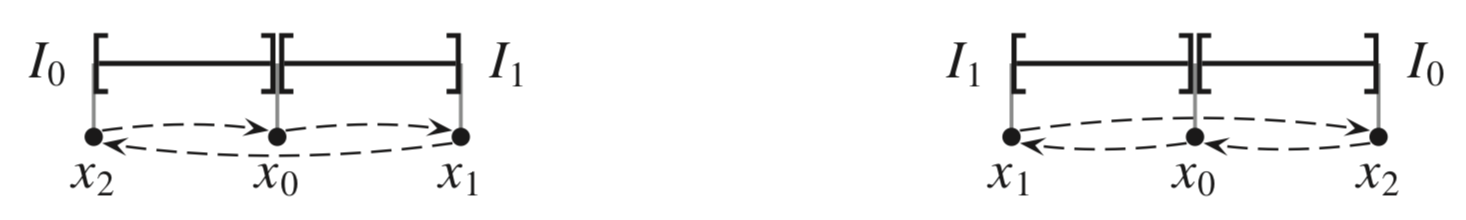
\includegraphics[scale=0.4]{sharkovsky1}
	\end{center}

Sea $I_{1}$ el intervalo con puntos extremos $x_{0}$ y $x_{1}$. Sea $I_{0}$ el intervalo con extremos $x_{0}$ y $x_{2}$. Tenemos que
	$$I_{1} \to I_{1}, \qquad I_{1} \to I_{0}$$

Consideremos el siguiente loop:
	$$I_{0} \to \underbrace{I_{1} \to \cdots \to I_{1}}_{\ell-1 \text{ copias}} \to I_{0} $$

Ninguno de los puntos extremos de $I_{0}$ posee tres iterados consecutivos en $I_{1}$. Además
	$$\rmx{int}(I_{0}) \cap \left(\bigcup_{i=1}^{\ell -1} I_{1}\right) = \rmx{int}(I_{0}) \cap I_{1} = \emptyset$$

Por lo tanto, por el \reftarget{lemcharkovsky3}, el loop es elemental y por el \reftarget{lemcharkovsky2} existe un punto $x \in I_{0}$ tal que $f^{i}(x) \in I_{i}$, $i \in \{1, \ldots, \ell -1\}$ y $f^{\ell}(x) = x$. En particular, $x$ tiene periodo $\ell$ y como $\ell$ es arbitrario, obtenemos lo pedido.
\end{proof}

\begin{defn}[Orden Sharkovsky] Consideremos el siguiente orden de los números naturales:
	$$\begin{array}{ccccccccccc}
		3			&	>	&	5			&	>	&	7			&	>	&	9			&	>	&	\cdots	&	>	&	\cdots	\\	
		2\cdot 3		&	>	&	2\cdot 5		&	>	&	2\cdot 7		&	>	&	2\cdot 9		&	>	&	\cdots	&	>	&	\cdots\\
		2^{2}\cdot 3	&	>	&	2^{2}\cdot 5	&	>	&	2^{2}\cdot 7	&	>	&	2^{2}\cdot 9	&	>	&	\cdots	&	>	&	\cdots\\
					&		&				&	\vdots&				&		&				&		&			&		&\\
		2^{n}\cdot 3	&	>	&	2^{n}\cdot 5	&	>	&	2^{n}\cdot 7	&	>	&	2^{n}\cdot 9	&	>	&	\cdots	&	>	&	\cdots\\
		\cdots		&	>	&	2^{n}			&	>	&	\cdots		&	>	&	2^{2}			&	>	&	2		&	>	&	1	
	\end{array}$$
\end{defn}

\begin{teo}[Sharkovsky '61] Sea $f: [a,b] \to [a,b]$ una función continua. Si $f$ posee una órbita periódica de periodo $\ell$ entonces $f$ posee órbita periódica de periodo $n$, con $n < \ell$ en el orden de Sharkovsky.
\end{teo}

\newpage
%%% Introducción a la teoría Ergódica %%%
\section{Introducción a la teoría Ergódica}

	%% Elementos de teoría de la medida %%
\subsection{Elementos de teoría de la medida}
\begin{defn} Sea $X$ conjunto. Una $\sigma$-álgebra $\clx{A}$ en $X$ es una colección de subconjuntos de $X$ tales que
	\begin{enumerate}[1)]
		\item $\emptyset, X \in \clx{A}$.
		\item Si $A \in \clx{A}$ entonces $A^{c} \in \clx{A}$.
		\item Si $\{U_{i}\}_{i \in \N}$ en $\clx{A}$, entonces $\bigcup_{i=1}^{\infty} U_{i} \in \clx{A}$.
	\end{enumerate}
\end{defn}

\begin{defn} Una función $\mu: \clx{A} \to \R^{+}$, donde $\clx{A}$ es una $\sigma$-álgebra de $X$ es una medida (en $X$) si
	\begin{enumerate}
		\item $\mu(\emptyset) = 0$.
		\item $A \subset B$ implica $\mu(A) \leq \mu(B)$.
		\item Si $\{A_{i}\}_{i \in \N} \subset \clx{A}$ son disjuntos, entonces
				$$\mu\left(\bigcup_{i \in \N} A_{i}\right) = \sum \mu(A_{i})$$
	\end{enumerate}
\end{defn}

\begin{defn} Si $\mu(X) < \infty$ entonces $\mu$ es una medida finita, mientras que si no, entonces $\mu$ es una medida infinita. Si además, $\mu(X) = 1$, entonces $\mu$ es una medida de probabilidad.
\end{defn}

	%% Definiciones %%
\subsection{Definiciones}
\begin{defn} Sea $T: X \to X$ y $\mu$ una medida en $X$. Diremos que $\mu$ es una medida $T$-invariante si para todo $A \in \clx{A}$ se tiene
	$$\mu(A) = \mu(T^{-1}A)$$
\end{defn}

\begin{obsd} Solo basta verificar la propiedad anterior en un álgebra que genera a $B$.
\end{obsd}

\begin{obsd} Si $\mu$ es $T$-invariante, la transformación $T$ preserva la estructura de espacio de medida de $(X, \clx{A}, \mu)$.
\end{obsd}

\begin{obsd} Si $\mu, \nu$ son $T$-invariantes, entonces para todo $\lambda \in [0,1]$ la medida
	$$\lambda\mu + (1-\lambda)\nu$$

es $T$-invariante.
\end{obsd}

\begin{ex} Toda rotación en $S^{1}$ preserva la medida de Lebesgue, pues esta es invariante bajo traslaciones (y las rotaciones de $S^{1}$ se pueden ver )
\end{ex}

\begin{ex} Sea 
	$$\func{T}{[0,1]}{[0,1]}
			{x}{2x \mod 1}$$
		
Y tomemos un intervalo $B$ y sus preimágenes, como en la figura
	\begin{center}
		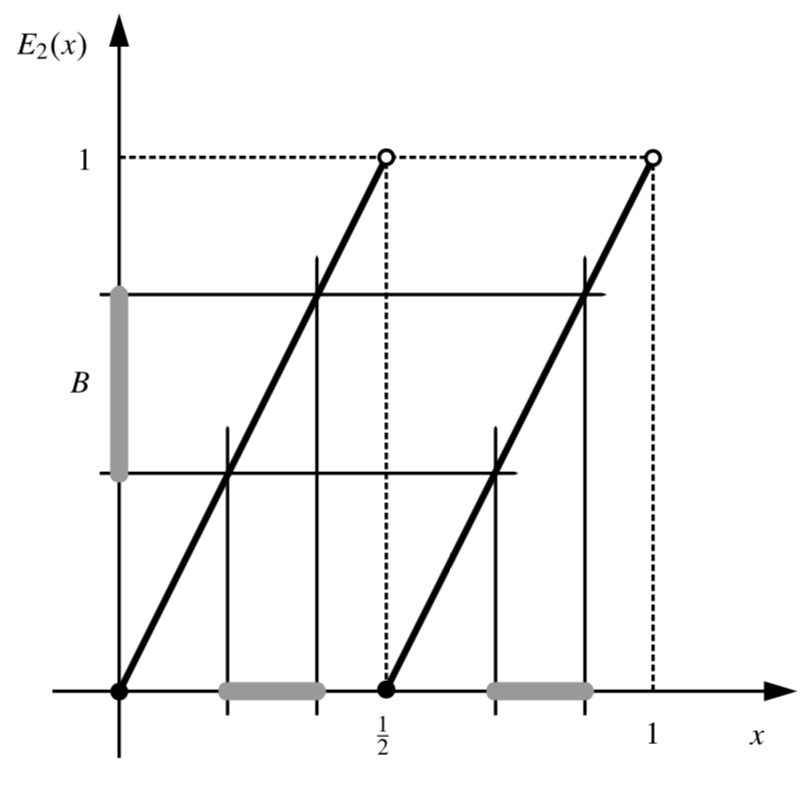
\includegraphics[scale=0.5]{por2mod1medida}
	\end{center}

Notar que cada uno de los intervalos marcados en el eje $x$ tiene la mitad del largo de $B$. Luego aquí la medida de Lebesgue $\lambda$ verifica
	$$\lambda(B) = \lambda(T^{-1}B)$$

por lo que $\lambda$ es $T$-invariante. Otra medida que es $T$-invariante en este caso es
	$$\delta_{0}(A) := \twodef{1}{0 \in A}
						{0}{0 \notin A}$$

Ocurre que para cada órbita periódica existe una medida invariante. Si tenemos
	$$x_{0} \tiende{T} x_{1} \tiende{T} x_{0}$$

entonces $\frac{\delta_{x_{0}} + \delta_{x_{1}}}{2}$ es $T$-invariante. En general si $\{x_{1}, \ldots, x_{n}\}$ es órbita periódica, entonces
	$$\delta = \frac{\delta_{x_{1}} + \cdots + \delta_{x_{n}}}{n}$$
\end{ex}

\begin{ex} Sea $(\Sigma, \sigma)$ el full shift en dos símbolos. Sea $p \in [0,1]$. Definimos la medida de Bernoulli $\mu_{p}$ de la siguiente manera:
	$$\mu_{p}([0]) = p, \qquad \mu_{p}([1]) = 1-p$$

y extendemos esta definición a todo cilindros como medida producto:
	$$\mu_{p}([a_{1} a_{2} a_{3} \cdots a_{n}]) = \prod_{j=1}^{n} \mu_{p}([a_{j}])$$

Luego, como los cilindros generan la $\sigma$-álgebra, obtenemos la medida. Notar que la medida $\mu_{p}$ es $\sigma$-invariante. En efecto, basta verificar en cilindros, si $I = [a_{1}a_{2} \cdots a_{n}]$, entonces
	$$\mu_{p}(I) = \prod_{i=1}^{n} \mu_{p}([a_{i}])$$

y como $\sigma^{-1}(I) = [0a_{1}a_{2}\cdots a_{n}] \cup [1a_{1}a_{2} \cdots a_{n}]$ y son disjuntos,
	$$\mu_{p}(\sigma^{-1}(I))
		=	\mu_{p}([0a_{1}a_{2} \cdots a_{n}]) + \mu_{p}([1 a_{1} a_{2} \cdots a_{n}])
		=	\mu_{p}([0])\mu_{p}(I) + \mu_{p}([1])\mu_{p}(I)
		=	\mu_{p}(I)$$
\end{ex}

\begin{ex} Sea $(\Sigma, \sigma)$ el full shift en dos símbolos y $\clx{T}: \Sigma \to \R$ una función continua y positiva. Sea $Y = \{(x,t) : x \in \Sigma, 0 \leq t \leq \clx{T}(x)\}$. Sea $\sim$ definida por
	$$(x, \clx{T}(x)) \sim (\sigma x, 0)$$

Sobre $\faktor{Y}{\sim}$ definimos el flujo de suspensión $\Phi = (\phi_{t})_{t \geq 0}$ por
	$$\phi_{t}(x,s)  = (x, s+t), \qquad \text{ si } 0 \leq s + t \leq \clx{T}(x)$$

En particular, se puede probar que si $\clx{M}_{\sigma}$ denota el espacio de las medidas de probabilidad $\sigma$-invariantes y $\clx{M}_{\phi}$ las invariantes por el flujo, entonces
	$$\func{R}{M_{\sigma}}{M_{\Phi}}
			{\mu}{\frac{\mu \times \lambda}{(\mu \times \lambda)(Y)}}$$
		
donde $\lambda$ es la medida de Lebesgue, es una biyección. Este es un resultado de Ambrose y Kakutani.
\end{ex}

\begin{ex} Sea $G: (0,1] \to (0,1]$ la transformación de Gauss:
	$$G(x) = \frac{1}{x} - \left[\frac{1}{x}\right]$$

con gráfico
	\begin{center}
		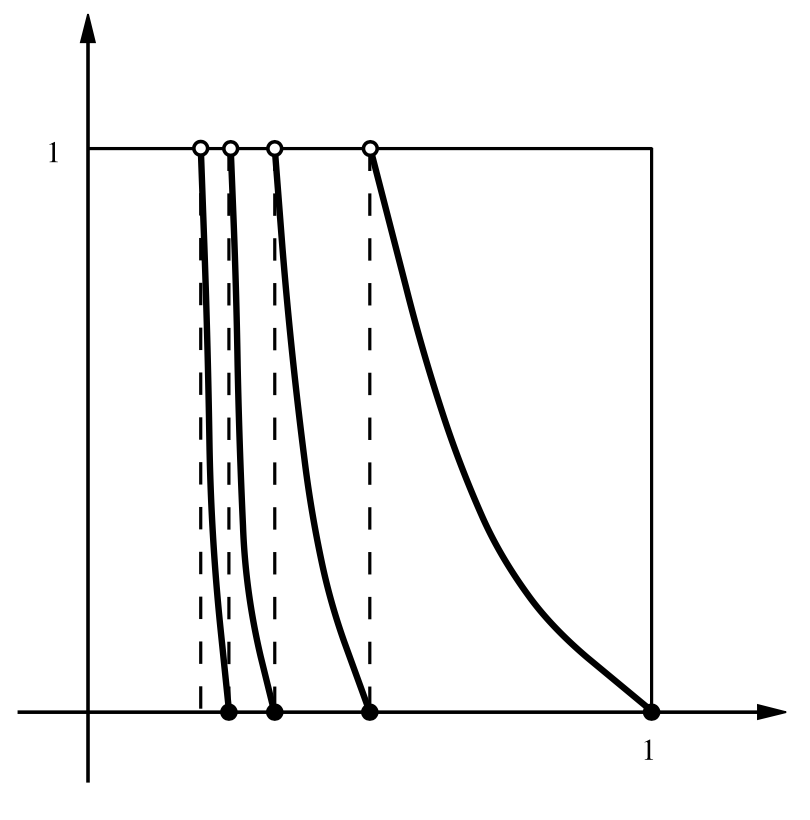
\includegraphics[scale=0.5]{transformaciongauss}
	\end{center}

La siguiente medida
	$$\mu_{G}(A) = \frac{1}{\ln 2} \int_{A} \frac{dx}{1+x}$$
	
es $G$-invariante.
\end{ex}

\begin{teo}[Teorema de recurrencia de Poincaré (1889)] Sea $T: X \to X$ y $\mu$ una medida finita $T$-invariante. Si $\mu(A) > 0$, entonces el conjunto
	$$B = \conj{x \in A}{\existe (n_{i})_{i \in \N} \text{ sucesión}, T^{n_{i}}(x) \in A}$$

es tal que $\mu(B) = \mu(A)$.
\end{teo}

\begin{proof}[Idea de la demostración] Sea $A \subset X$ con $\mu(A) > 0$. Si los conjuntos $A, T^{-1}A, T^{-2}A, \ldots, T^{-n}A$ son dos a dos disjuntos, entonces, como $\mu$ es $T$-invariante, entonces
	$$\mu(A) = \mu(T^{-1}A) = \mu(T^{-2}A) = \cdots = \mu(T^{-n}A), \qquad \paratodo n \in \N$$
			
Así, como $\mu(A) > 0$
	$$1 = \mu(x) \geq \mu\left(\bigcup_{n=1}^{\infty} T^{-n}A\right) = \sum_{n=1}^{\infty} \mu(A) = \infty$$

Lo que es una contradicción, luego existen $m,n \in \N$ tales que
	$$T^{-m}A \cap T^{-n}A \neq \emptyset$$
	
y
	$$\mu(T^{-m}(A \cap T^{-m-n}A)) = \mu(A \cap T^{-m-n}A)$$

\end{proof}

\begin{ex} Sea $A$ el conjunto de los números cuya expansión en base 3 comienza con 0. Como la medida de Lebesgue es $T$-invariante, el teorema de recurrencia de Poincaré implica que casi todos los números cuya expansión en base 3 comienza en 0 son tales que el dígito 0 aparece infinitas veces en su expansión. En este caso, $T$ es $3x \mod 1$.
\end{ex}

	%% Teoremas Ergódicos %%
\subsection{Teoremas Ergódicos}

\begin{defn}Sea $T: X \to X$. Un subconjunto $A \subset X$ es $T$-invariante si $A = T^{-1}A$.
\end{defn}

\begin{obsd} Si $A$ es $T$-invariante, entonces $X \setminus A$ también lo es. Por lo tanto, en vez de estudiar la dinámica de $T$ en $X$, es más simple estudiar independientemente los sistemas $T: A \to A$ y $T: X \setminus A \to X \setminus A$.
\end{obsd}

\begin{ex} Yan hemos visto el sistema dinámico
	\begin{center}
		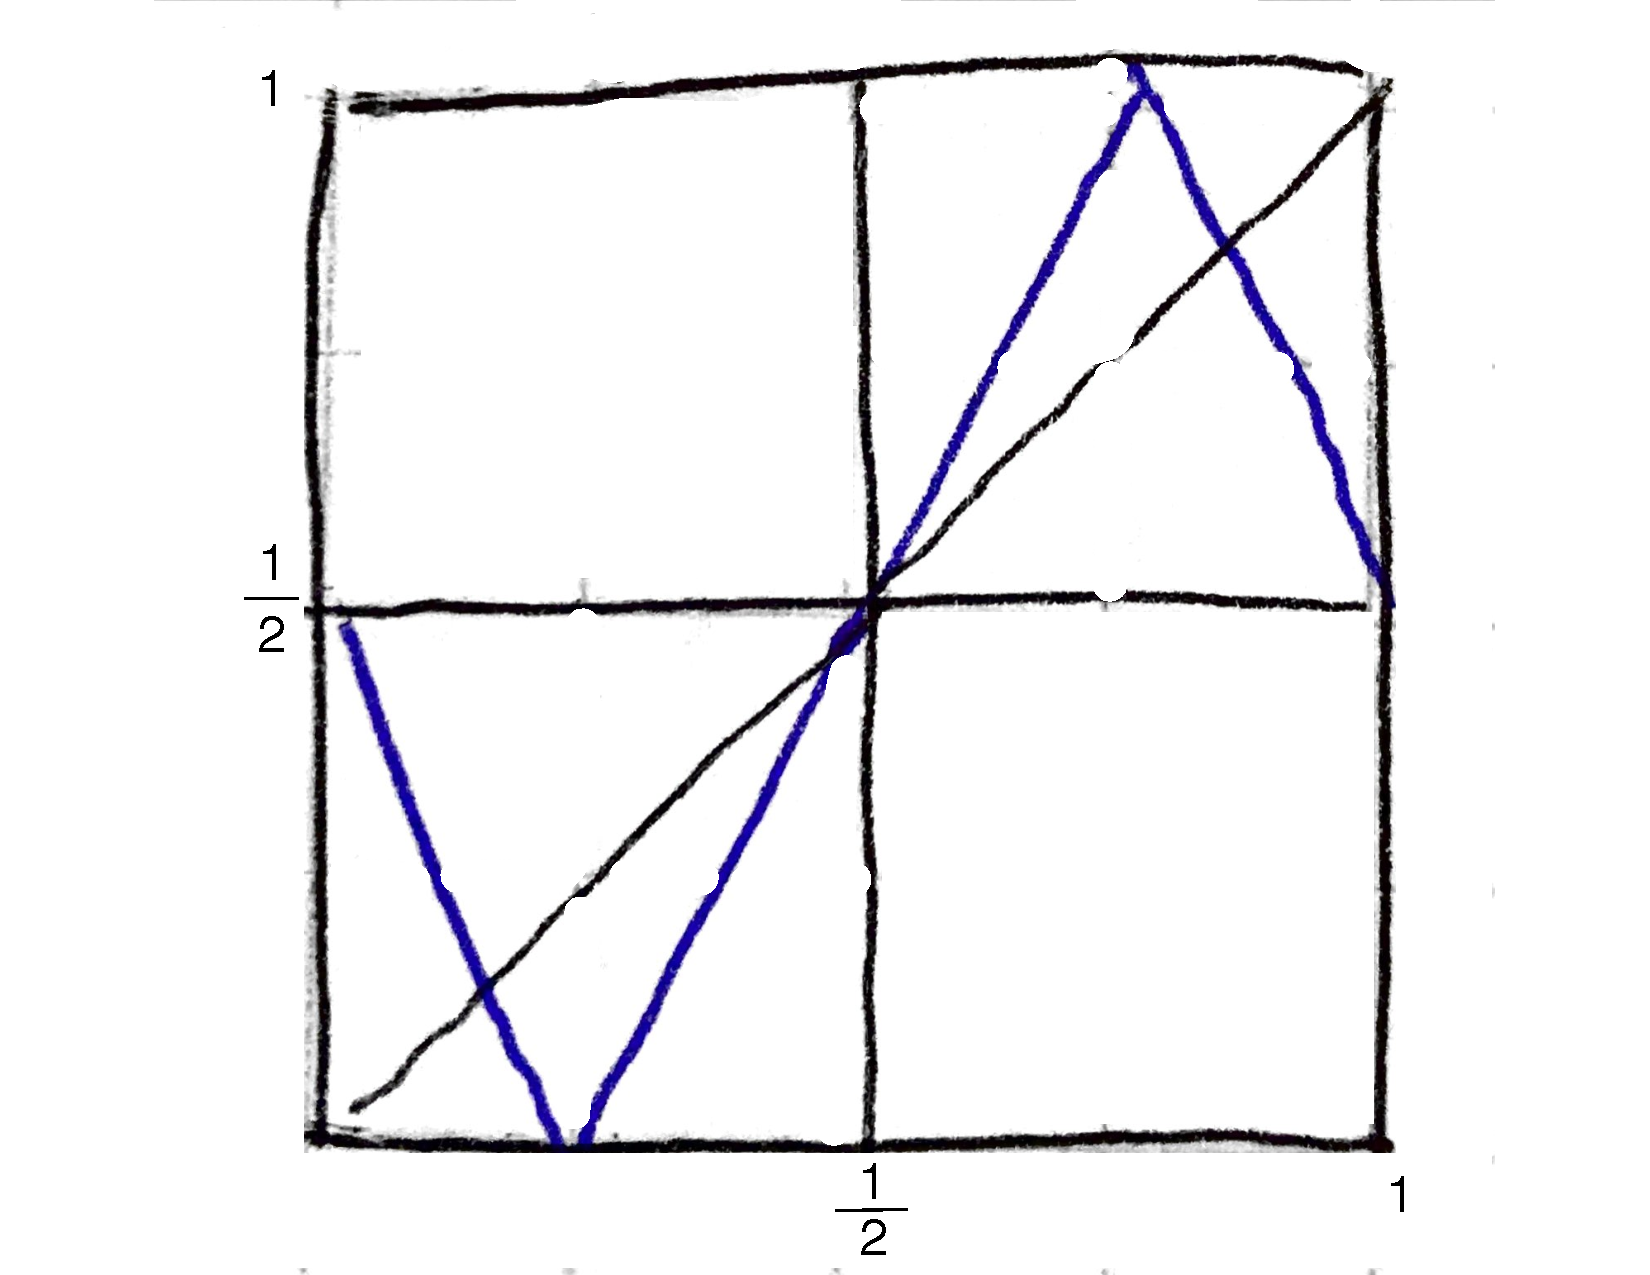
\includegraphics[scale=0.24]{dibujo1}
	\end{center}

en el cual podemos mirar $T: \left[0,\frac{1}{2}\right] \to \left[0,\frac{1}{2}\right]$ y $T: \left[\frac{1}{2}, 1\right] \to \left[\frac{1}{2}, 1\right]$.
\end{ex}

\begin{defn} Una medida $T$-invariante, $\mu$, es \rojo{ergódica} si para todo conjunto invariante $A$ se tiene
	$$\mu(A) = 0 \quad \text{ó} \quad \mu(A) = 1$$
\end{defn}

\begin{ex} \quad
\begin{enumerate}[\indent 1)]
	\item La medida de Lebesgue es ergódica para toda rotación irracional.
	\item Las medidas de Bernoulli, $\mu_{p}$, son ergódicas en $\Sigma_{2}$.
	\item La medida de Gauss es ergódica con respecto a la transformación de Gauss.
	\item Si $\mu$ es ergódica con respecto a $(\Sigma, \sigma)$, entonces $\mu \times \lambda$ (con $\lambda$ la medida de Lebesgue) es ergódica con respecto al flujo de suspensión asociado (para todo techo continuo $\clx{T}$).
	\item La medida de Lebesgue es ergódica con respecto a $T(x) = mx \mod 1$. La medida atómica en 0 también es ergódica en este caso.
\end{enumerate}
\end{ex}

Sea $T: X \to X$ continua y $X$ compacto. Entonces el espacio de medida de probabilidad $T$-invariantes, $M$, es convexo y compacto. Donde la topología usada es la $\Asterisk$-débil, lo que significa que $\{\mu_{n}\}_{n \in \N} \subset M$ converge $\Asterisk$-débilmente a $\lambda$ si
	$$\lim_{n \to \infty} \int f \, d\mu_{n} = \int f \, d\mu, \qquad \paratodo f \in C(X)$$

Además, se tiene que todo punto extremo de $M$, es decir, tal que no puede escribirse como combinación lineal convexa de otras medidas, es ergódico. Observar en particular que si $M = \{\mu\}$, entonces $\mu$ es ergódica.

Ahora, consideremos $T: X \to X$ y $\mu$ ergódica tal que para todo abierto $A \subset X$, $\mu(A) > 0$. Entonces existe una órbita densa en $X$.

		%	Teorema de Birkhoff %
\subsubsection{Teorema de Birkhoff}
Sea $f: [a,b] \to \R$ una función integrable. Sea
	$$F(x) = \int_{a}^{x} f(y) \, dy, \qquad F: [a,b] \to \R$$ 

Luego,
	$$F'(x) = \lim_{h \to 0^{+}} \frac{F(x+h)- F(x)}{h} = \lim_{h \to 0^{+}} \frac{1}{h} \int_{x}^{x+h} f(y) \, dy$$

La pregunta ahora es cuándo ocurre que
	$$\lim_{h \to 0} \frac{1}{h} \int_{x}^{x+h} f(y) \, dy$$

Para resolver este problema. Nos interesa estudiar lo siguiente. Dada $(S_{n})_{n}$ una sucesión de operadores en $L^{1}(\mu)$ queremos saber cuándo o cómo, la sucesión $(S_{n}f)(x)$ converge en casi todo punto $x$ para $f \in L^{1}(\mu)$. Es decir, cuándo o cómo podemos probar que $(S_{n}f(x))_{n}$ es sucesión de Cauchy en casi todo punto. Esto quiere decir que si $f \in L^{1}(\mu)$ y $\alpha > 0$,
	$$\mu\left(\conj{x \in X}{\limsup_{n,m \to \infty} |(S_{n}f)(x) - (S_{m}f)(x)| > \alpha}\right) = 0$$

Asumamos que existe un conjunto $\clx{C} \subset L^{1}(\mu)$ tal que $\clx{C}$ es denso y para toda $f \in \clx{C}$, $(S_{n}f)(x)$ converge en todo punto $x \in X$. Sea $f \in L^{1}(\mu)$ y $\epsilon > 0$, entonces existe $g \in \clx{C}$ y $h_{\epsilon} \in L^{1}(\mu)$ tal que
	$$f = g + h_{\epsilon}, \qquad \|h_{\epsilon}\|_{1} < \epsilon$$

Luego
	\begin{align*}
		&\conj{x \in X}{\limsup_{n,m \to \infty} |(S_{n}f)(x) - (S_{m}f)(x)| > \alpha}	\\
			&\qquad =		\conj{x \in X}{\limsup_{n,m \to \infty} |(S_{n}g)(x) - (S_{m}g)(x)| > \frac{\alpha}{2}}	\\
			&\qquad \subset	\conj{x \in X}{\limsup_{n,m \to \infty} |(S_{n}g)(x) - (S_{m}g)(x)| > \frac{\alpha}{2}} \cup \conj{x \in X}{\limsup_{n,m \to \infty} |(S_{n}h_{\epsilon})(x) - (S_{m}h_{\epsilon})(x)| > \alpha}
	\end{align*}

Luego
	$$\mu\left(\conj{x \in X}{\limsup_{n,m \to \infty} |(S_{n}g)(x) - (S_{m}g)(x)| > \frac{\alpha}{2}}\right) = 0$$

y por otro lado, usando que
	\begin{align*}
		\alpha
			&\leq		\limsup_{n,m \to \infty} |S_{n}h_{\epsilon}(x) - S_{m}h_{\epsilon}(x)|	\\
			&\leq		\sup_{n,m} |S_{n}h_{\epsilon}(x) - S_{m}h_{\epsilon}(x)|		\\
			&\leq		\sup_{n,m} \{ |S_{n}h_{\epsilon}(x)| + |S_{m}h_{\epsilon}(x)|  \}	\\
			&\leq		\sup_{n} |2S_{n}h_{\epsilon}(x)|
	\end{align*}

Entonces
	\begin{align*}
		\conj{x \in X}{\limsup_{n,m \to \infty} |S_{n}h_{\epsilon}(x) - S_{m}h_{\epsilon}(x)| > \alpha}
			&\subseteq	\conj{x \in X}{\sup_{n} 2|S_{n}h_{\epsilon}(x)| > \alpha}	\\
			&=			\conj{x \in X}{\sup_{n} |S_{n}h_{\epsilon}(x)| > \frac{\alpha}{2}}
	\end{align*}

Si $\|h_{\epsilon}\| \to 0$, entonces
	$$\mu\left(\conj{x \in X}{\sup_{n} |S_{n}h_{\epsilon}(x)| > \alpha}\right) = 0$$

Estudiaremos entonces el operador
	$$S^{*}f(x) = \sup_{n} |S_{n}f(x)|$$

Observemos que si existera $c > 0$ tal que para todo $f \in L^{1}(\mu)$, 
	$$\|S^{*}f\|_{1} \leq c\|f\|_{1}$$

entonces el problema estaría terminado. Sin embargo, en general, $S^{*}f \notin L^{1}(\mu)$ (de hecho la desigualdad anterior vale para toda $f \in L^{p}$ y usando la norma $p$, con $p > 1$). Sin embargo, si existe $c > 0$ tal que para todo $f \in L^{1}(\mu)$ se tiene
	$$\mu\left(\conj{x \in X}{S^{*}f(x) > \alpha}\right) \leq \frac{c\|f\|_{1}}{\alpha}$$

entonces estamos listos. Este procedimiento se conoce como \rojo{principio de Banach} que dice que si tenemos un denso $\clx{C}$ que cumple la convergencia y se cumple la desigualdad anterior, entonces $S_{n}f(x)$ converge en casi todo punto.

\begin{teo}[Vitali] Sea $\clx{B} = \{B_{1}, \ldots, B_{N}\}$ una colección de bolas abiertas en $\R^{d}$. Entonces existe una sub-colección disjunta de $\clx{B}$, $\{B_{i_{1}}, \ldots, B_{i_{k}}\}$ tal que
	$$\lambda\left(\bigcup_{\ell=1}^{N} B_{\ell}\right) \leq 3^{d}\sum_{j=1}^{k} \lambda(B_{i_{j}})$$
\end{teo}

\begin{defn}[Función maximal de Hardy-Littlewood] Sea $f \in L^{1}(\lambda)$ (con $\lambda$ la medida de Lebesgue). La función maximal asociada se define por
	$$f^{*}(x) := \sup_{B \ni x} \frac{1}{\lambda(B)} \int_{B} |f(y)| \,dy$$
\end{defn}

\begin{teo} Sea $f \in L^{1}(\lambda)$, entonces
	\begin{enumerate}[\indent 1)]
		\item $f^{*}$ es medible.
		\item $f^{*}(x) <\infty$, $\lambda$-ctp.
		\item $\lambda(\{x \in \R^{d} : f^{*}(x) > \alpha\}) \leq \frac{A}{\alpha} \|f\|_{L^{1}}$.
	\end{enumerate}
\end{teo}

\begin{proof}[Demostración de 3)] Sea $K \subset E_{\alpha} := \{x \in \R^{d} : f^{*}(x) > \alpha\}$, compacto. Claramente
	$$K \subset \bigcup_{x \in E_{\alpha}} B_{x}$$

donde cada bola $B_{x}$ es tomada de manera que
	$$f^{*}(x) 
		=	\sup_{B \ni x} \frac{1}{\lambda(B)} \int_{B} |f(y)| \, dy 
		\geq	\frac{1}{\lambda(B_{x})} \int_{B_{x}} |f(y)| \, dy
		>	\alpha
	$$

lo que puede hacerse por definición de supremo. Como $K$ es compacto, escogemos un subcubrimiento finito,
	$$K \subset \bigcup_{\ell=1}^{N} B_{\ell}$$

Por el teorema de Vitali, existe $\{B_{i_{1}}, \ldots, B_{i_{k}}\}$ tal que
	$$\lambda\left(\bigcup_{\ell=1}^{N} B_{\ell}\right) \leq 3^{d} \sum_{j=1}^{k} \lambda(B_{i_{j}})$$

Luego, como 
	\begin{align*}
		\lambda(K) 
			&\leq		3^{d} \sum_{j=1}^{k} \lambda(B_{i_{j}})	\\
			&\leq		\frac{3^{d}}{\alpha}\sum_{j=1}^{k} \int_{B_{i_{j}}} |f(y)| \, dy	\\
			&\leq		\frac{3^{d}}{\alpha} \int_{\bigcup_{j=1}^{k} |f(y)| \, dy}	\\
			&\leq		\frac{3^{d}}{\alpha}\|f\|_{1}
	\end{align*}


\end{proof}

\begin{teo}[Lebesgue, 1910] Sea $f \in L^{1}(\lambda)$, con $\lambda$ la medida de Lebesgue, entonces
	$$\lim_{h \to 0} \frac{1}{h} \int_{x}^{x+h} f(y) \, dy = f(x)$$

$\lambda$-ctp en $x$.
\end{teo}

\begin{proof} (Hardy-Littlewood) Si $f$ es continua, el resultado sigue directamente del TFC. Notemos que el espacio de las funciones continuas es denso en $L^{1}(\lambda)$. Queremos entonces ocupar el principio de Banach, con la función maximal definida anteriormente. El teorema anterior dice que se verifica la desigualdad deseada y con eso concluimos la convergencia.
\end{proof}

\begin{teo}[Teorema maximal ergódico] Si $f \in L^{1}(\mu)$ y 
	$$f^{*}(x) := \sup_{1 \leq n < \infty} \frac{1}{n} \sum_{i=1}^{n-1} |f(T^{i}x)|$$

entonces
	\begin{enumerate}[(i)]
		\item $\mu$-ctp, $f^{*} < \infty$.
		
		\item Existe $A > 0$, tal que para todo $\alpha > 0$
				$$\mu\left(\conj{x \in X}{f^{*}(x) > \alpha}\right) \leq \frac{A}{\alpha}\|f\|_{1}$$
	\end{enumerate}
\end{teo}

\begin{proof} (Tarea I3) Revisar 
	\begin{enumerate}
		\item Ergodic Theory, Walters (A. Garsia).
		\item Real Analysis, Stein \& zxShakarchi.
		\item Ergodic Theory, Petersen.
	\end{enumerate}
\end{proof}


\begin{teo}[Birkhoff] Sea $T: X \to X$ y $\mu$ una medida $T$-invariante ergódica. Si $f \in L^{1}(\mu)$, entonces
	$$\lim_{n \to \infty} \frac{1}{n} \sum_{i=0}^{n-1} f(T^{i}x) = \int f \, d\mu$$ 
\end{teo}

\begin{proof} Sea
	$$I = \conj{f \in L^{1}(\mu)}{f \circ T = f}$$

Notar que para cada $f \in I$
	$$\lim_{n \to \infty} \frac{1}{n} \sum_{i=0}^{n-1} f(T^{i}) 
		= \lim_{n \to \infty} \frac{1}{n} \sum_{i=0}^{n-1} f 
		= f
	$$

Sea $\clx{C} = \{f - f \circ T : f \in L^{1}(\mu)\}$. Notar que, si llamamos $S = \frac{1}{n} \sum_{i=0}^{n-1} f(T^{i})$,
	\begin{align*}
		S
			&=	\frac{1}{n} (f(x) - f(Tx) + f(Tx) - f(T^{2}x) + f(T^{2}x) - \cdots + f(T^{n-1}x) - f(T^{n}x))	\\
			&=	\frac{1}{n}(f(x) - f(T^{n}x))
	\end{align*}

Luego, si $n \to \infty$, $\frac{1}{n} f(x) \to 0$, por lo que basta analizar que ocurre con
	$$\lim_{n \to \infty} \frac{f(T^{n}(x))}{n}$$

Queremos probar que ese límite es 0. Recordemos que si tenemos una sucesión de funciones $a_{k}(x) \geq 0$, entonces el teorema de convergencia monótona dice que si
	$$\sum_{k=1}^{\infty} \int a_{k}(x) \, dx$$

converge, entonces
	$$\sum_{k=1}^{\infty} a_{k}(x)$$

converge $\mu$-ctp. Notemos que
	$$\sum_{k=1}^{\infty} \frac{1}{k^{2}} \int (f(T^{k}(x)))^{2} \, d\mu
		=	\sum_{k=1}^{\infty} \frac{1}{k^{2}} \| f \circ T^{k}\|^{2}_{2}
	$$

Como la medida $\mu$ es $T$-invariante, para toda $f \in L^{1}(\mu)$,
	$$\int f \, d\mu = \int (f \circ T^{k}) \, \mu, \qquad \paratodo k \in \N$$

Luego, para todo $k \in \N$,
	$$\|f \circ T^{k}\|_{2} = \|f\|_{2}$$

Así, 
	$$\sum_{k=1}^{\infty} \frac{1}{k^{2}} (f \circ T^{k})^{2}$$

converge $\mu$-ctp. Luego
	$$\lim_{k \to \infty} \frac{(f(T^{k}x))^{2}}{k^{2}} = 0$$
	
mostrando lo pedido. De esta forma, tenemos que el teorema se cumple en
	$$B = \conj{h_{1} + h_{2}}{h_{1} \in L^{2}(\mu) \cap I, \, h_{2} \in L^{2}(\mu) \cap \clx{C}}$$

Pero sucederá que $B$ es (casi) denso en $L^{2}(\mu)$ y como además $L^{2}(\mu)$ es denso en $L^{1}(\mu)$, entonces se tiene lo pedido, pues para $f \in L^{1}(\mu)$, la función maximal
	$$f^{*}(x) := \sup_{1\leq n < \infty} \frac{1}{n} \sum_{i=1}^{n-1} |f(T^{i}x)|$$

del teorema anterior verifica la desigualdad necesaria para aplicar el principio de Banach.	\\

Volviendo a la demostración de la densidad, sucederá que el conjunto que es denso es
	$$\tilde{B} = I + \overline{\clx{C}}$$

de manera que toda $f \in L^{1}(\mu)$ se puede escribir como
	$$f = h_{1} + h_{2} + e$$

donde $h_{1} \in I, h_{2}, e \in \clx{C}$ y $\|e\|$ es suficientemente chica.

\begin{ej} Suponiendo el Teorema maximal ergódico y que el conjunto $\tilde{B}$ es denso en $L^{1}(\mu)$. Demuestre luego que $\mu$-ctp
	$$\lim_{n \to \infty} \sum_{i=0}^{n-1} f(T^{i}x)$$

converge.
\end{ej}
 
\end{proof}

\begin{cor} Sea $A$ un conjunto medible tal que $\mu(A) > 0$. Entonces
	$$\lim_{n \to \infty} \frac{1}{n}\, \#\{i \in \{0, \ldots, n-1\} : T^{i}x \in A\} = \mu(A)$$
\end{cor}

		%	Teorema ergódico de von Neumann %
\subsubsection{Teorema ergódico de von Neumann}
\begin{defn} Sea $T: X \to X$ y $\mu$ una probabilidad $T$-invariante. Se define el operador de Koopman por
	$$\func{U}{L^{2}(\mu)}{L^{2}(\mu)}
			{f}{f \circ T}$$
\end{defn}

\begin{obsd} El operador $U$ está bien definido, es decir $U(f) \in L^{2}(\mu)$ para toda $f \in L^{2}(\mu)$ pues $\mu$ es $T$-invariante y por lo tanto
	$$\int f \, d\mu = \int f \circ T \, d\mu$$
\end{obsd}

\begin{lem} El operador de Koopman es una isometría lineal, es decir, $U$ es lineal y
	$$\|U(f)\| = \|f\|$$
\end{lem}

\begin{proof} La linealidad es clara y la isometría sigue de la observación:
	\begin{align*}
		\|f\|_{2}
			&=	\left(\int |f|^{2} \, d\mu\right)^{1/2}	\\
			&=	\left(\int |f \circ T|^{2} \, d\mu\right)^{1/2}	\\
			&=	\|f \circ T\|_{2}
	\end{align*}
\end{proof}

\begin{teo}[von Neumann / Carleman] Sea $T : X \to X$ una transformación que preserva la medida de probabilidad $\mu$. Si $f \in L^{2}(\mu)$ entonces existe $f^{*} \in L^{2}(\mu)$ tal que
	$$f^{*} \circ T = f^{*}$$
	
y
	$$\lim_{n \to \infty} \left\| \frac{1}{n} \sum_{i=0}^{n-1} f(T^{i}x) - f^{*}(x)\right\|_{2} = 0$$  
\end{teo}




\end{document}